\documentclass[preprint]{aastex}
\usepackage{amsmath}
\usepackage{newtxtext, newtxmath}
\usepackage{booktabs}
\usepackage{graphicx}
\graphicspath{
  {../},
}


\usepackage{geometry}
\geometry{margin=1in}
\setkeys{Gin}{width=0.6\linewidth, keepaspectratio}  

\usepackage{natbib}
\usepackage{microtype}
\usepackage{xcolor}
\bibliographystyle{apj}


\newcommand\Pixel{\ensuremath{\Omega_{\mathrm{pix}}}}
\newcommand\Area{\ensuremath{A_{\mathrm{HST}}}}
\newcommand\T[2]{\ensuremath{T_{#1}^{#2}}}
\newcommand\Tlam[1]{\T{\lambda}{#1}}
\newcommand\Tmax[1]{\T{\mathrm{m}}{#1}}
\newcommand\Mean[1]{\ensuremath{\bigl\langle \lambda I_\lambda \bigr\rangle_{#1}}}
\newcommand\MeanC[1]{\ensuremath{\bigl\langle \lambda
    I_\lambda^{\mathrm{cont}} \bigr\rangle_{#1}}}
\newcommand\Color[2]{\ensuremath{k_{#1, #2}}}
\newcommand\COLOR[2]{\ensuremath{\widetilde{k}_{#1, #2}}}
\newcommand\Weff[2]{\ensuremath{\widetilde{W}_{#1, #2}}}
\newcommand\U[1]{\ensuremath{\mathrm{#1}}}
\newcommand\E[1]{\ensuremath{\times 10^{#1}}}
\newcommand\Elam{\ensuremath{\varepsilon_\lambda}}
\newcommand\Constant{\ensuremath{C_{\mathrm{WFC3}}}}


% \newcommand\Narrow{\mathrm{L}}
% \newcommand\Wide{\mathrm{C}}
% \newcommand\Narrow{\mathrm{a}}
% \newcommand\Wide{\mathrm{b}}
\newcommand\Narrow{\mathrm{N}}
\newcommand\Wide{\mathrm{W}}
\newcommand\Contam{\ensuremath{{i'}}} %extra braces are on purpose



\begin{document}
\title{Temperature and density fluctuations in the inner Orion Nebula}
\author{W. J. Henney, C. R. O'Dell, G. J. Ferland, M. Peimbert}
\section{Analysis}
\label{sec:fluct}



\subsection{Deriving diagnostic line ratios from WFC3 filter images}
\label{sec:filters}
% \begin{figure}
%   \centering
%   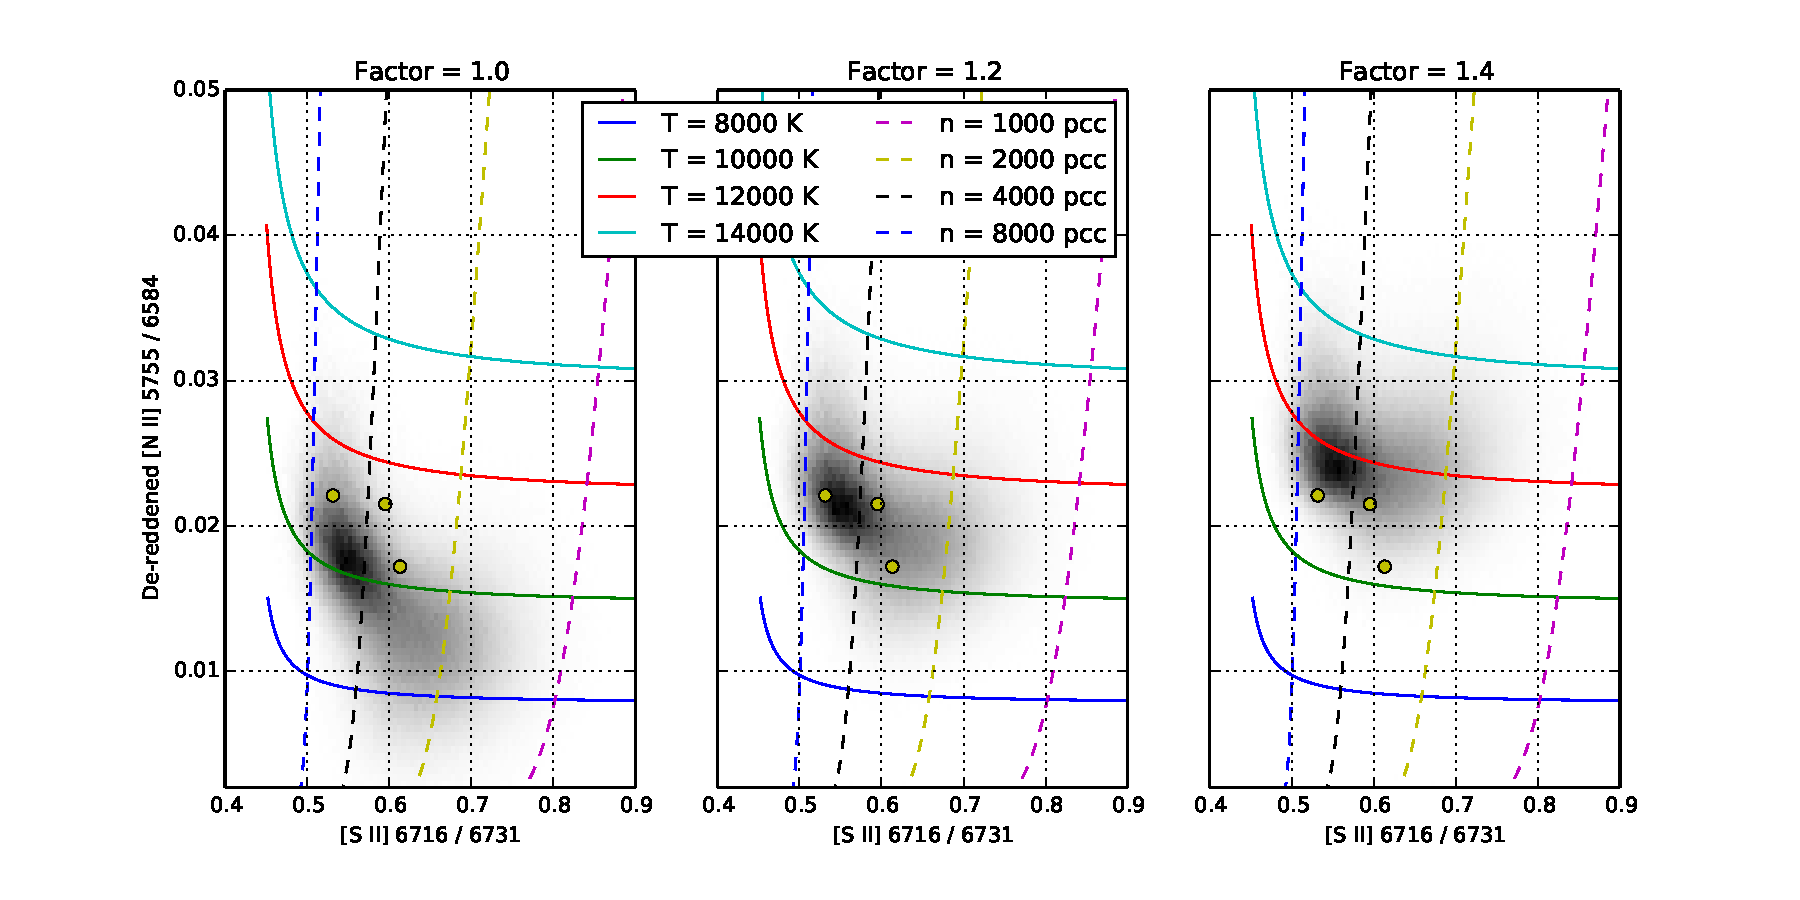
\includegraphics[width=\linewidth]{bivar_rsii_rnii_multifactor}
%   \caption{Distribution of line ratios}
%   \label{fig:line-ratios}
% \end{figure}

\textit{Note: this is similar to what I wrote in the the calibration
  draft, but specifically tailored to line ratios rather than
  equivalent widths.  We may in the end want to move some of it back
  to the other paper.}

The WFC3 camera is equipped with filters that effectively target
important nebular diagnostic lines.  Each filter, with label \(j\), is
characterized by an effective transmission profile, or throughput,
\Tlam{j}, which gives the wavelength-dependent conversion factor
between the number of photons arriving at the \textit{HST} entrance
aperture (nominal radius: \(120\ \U{cm}\)) and the number of electrons
registered by the CCD, accounting for occultation by the secondary
mirror, all other optical and quantum efficiencies, and the amplifier
gain.  The peak value of the filter transmission profile is denoted
\Tmax{j}, with typical values of 0.2--0.3, and the ``rectangular
width'' of the profile is defined as
\begin{equation}
  \label{eq:width}
  W_j = (\Tmax{j})^{-1} \int_0^\infty \!\!\Tlam{j}\, d\lambda 
  \quad\quad [W_j] = \U{\AA}.
\end{equation}


Extensive and continuing on-orbit calibration of the filters has been
carried out \citep{Kalirai:2009a, Kalirai:2010a, Sabbi:2013b} using
white dwarf standard stars.  However, since these are flat featureless
continuum sources, the calibration is only sensitive to the integrated
filter throughput, given by the product \(W_j \Tmax{j}\).  A general
increase in the integrated throughput of 10--20\% with respect to
pre-launch measurements was found for all filters, which was fitted by
a low-order polynomial as a function of frequency.  Only the
broad-band and medium-band filters were used in determining the fit,
but the scatter of the narrow-band filters\footnote{Note, however,
  that the quad filters were not included in these studies.} around
the resulting curve is only a few percent (see Fig.~6 of
\citealp{Kalirai:2009a}).

Emission lines from photoionized regions are intrinsically much
narrower than even the narrowest WFC3 filters, so the transmission of
such a line, with label \(i\), is independent of \(W_j\) and depends
instead solely on the throughput at the line wavelength: \(\T{i}{j}
\equiv \Tlam{j}(\lambda\!=\!\lambda_i)\).  The detailed shape of the
throughput curves was measured pre-launch \citep{Brown:2006a}, but
direct on-orbit confirmation of these curves is impossible.  However,
by comparing WFC3 images with ground-based spectrophotometry of
emission line nebulae, it is possible to test the filter calibrations
for the case where emission lines are the dominant component of the
spectrum in the filter bandpass.  Just such a calibration is described
in detail in a companion paper \citep{Henney:Calibration}, using
multiple spectrophotometric datasets of the Orion Nebula (M42) and the
evolved nearby planetary nebula NGC~6720 (the Ring Nebula), and
building on an earlier study in \citet{ODell:2013b}.  The conclusion
of this study is that the nominal filter parameters (that is, the
pre-launch measurements of the shape of the throughput curve \Tlam{j},
combined with the on-orbit re-calibration of \(W_j \Tmax{j}\)), are
consistent to within \(\pm 5\%\) with the emission line
spectrophotometry for all but a handful of filters.  The largest
discrepancy is found for the F469N filter, which is found to have a
sensitivity to the \ion{He}{2} \Wav{4686} line that is 35\% higher than the
nominal value.  However, that line is absent in M42, due to the
relatively low effective temperature of the ionizing star, and the
filter is instead dominated by continuum and weak [\ion{Fe}{3}]
lines.  In such circumstance the nominal F469N parameters are found to
be accurate.  

Smaller, but still significant, discrepancies are found for the F658N
and FQ575N filters, which target the \nii{} lines \Wav{6583} and
\Wav{5755}, respectively. \textit{Discuss inconsistency between Ring
  and Orion calibration.  Ring has 5755 increased by 10\%.  Orion has
  6583 decreased by 10\%.  But effects on ratio are similar.}

We model the specific intensity, \Ilam (in \U{erg\ s^{-1}\ cm^{-2}\
  sr^{-1}\ \AA^{-1}}), of a spatially resolved astrophysical source as
the sum of several narrow emission lines \(i\), each with central
wavelength \(\lambda_i\) and wavelength-integrated intensity \(I_i\),
plus a slowly varying continuum \Icont:
\begin{equation}
  \label{eq:line-plus-cont}
  \Ilam = \Icont + \sum_{i=1, n} I_i\, \delta(\lambda - \lambda_i)  ,
\end{equation}
where \(\delta\) denotes the Dirac delta function.   It is convenient
to define an average continuum intensity over the passband of filter \(j\): 
\begin{equation}
  \label{eq:average}
  \MeanC{j} = \int_0^\infty \!\!\lambda \Icont  \Tlam{j} \, d\lambda \,
  \Bigg/\! \int_0^\infty \!\!\Tlam{j} \, d\lambda .
\end{equation}
The count rate (in \U{e^-/s}) in a single pixel of a pipeline-reduced
(bias-subtracted, flat-fielded, drizzled) WFC3 image should then be
\begin{equation}
  \label{eq:R-line-plus-cont}
  R_j 
  = \Constant\,
  \left(
    \MeanC{j} \, \Tmax{j} W_j 
    + \sum_{i=1,n} \lambda_i I_i \T{i}{j}
  \right)
\end{equation}
where \(\Constant = 10^{-8} \Area\, \Pixel / (h c) = 0.0840241\
\U{counts\ cm^2\ sr\ erg^{-1}\ \AA^{-1}\ pixel^{-1}}\) is a constant
for the camera, depending on the telescope aperture area, \(\Area =
\pi (120\ \U{cm})^2 = 45,239\ \U{cm^2}\), and the solid-angle
subtended\footnote{Although geometric distorsions by the telescope
  optics mean that the true pixel area varies across the field of
  view, this is corrected for during the ``drizzle'' stage of the
  pipeline reduction process, which yields images (extension
  \texttt{drz}) interpolated onto a regular pixel grid.  If
  non-drizzled (extension \texttt{flt}) images are used, then a
  further correction for the pixel area map must be applied to
  equation~(\ref{eq:R-line-plus-cont}).} by each pixel \(\Pixel =
(0.03962'')^2 = 3.6895\E{-14}\ \U{sr}\).

% \newcommand\F[1]{%
%   \ifmmode{\scriptscriptstyle \mathrm{#1}}\else{\textsc{\lowercase{#1}}}\fi
% }
\newcommand\F[1]{%
  % \ifmmode\scriptsize\fi\textsc{\lowercase{#1}}
  \ifmmode\scriptscriptstyle\mathrm{#1}\else #1\fi
}
\newcommand\Falpha[1]{\ensuremath{\alpha_{\F{#1}}}}
\newcommand\Fbeta[1]{\ensuremath{\beta_{\F{#1}}}}
\newcommand\Fgamma[1]{\ensuremath{\gamma_{\F{#1}}}}

\begin{figure}[t]
  \centering
  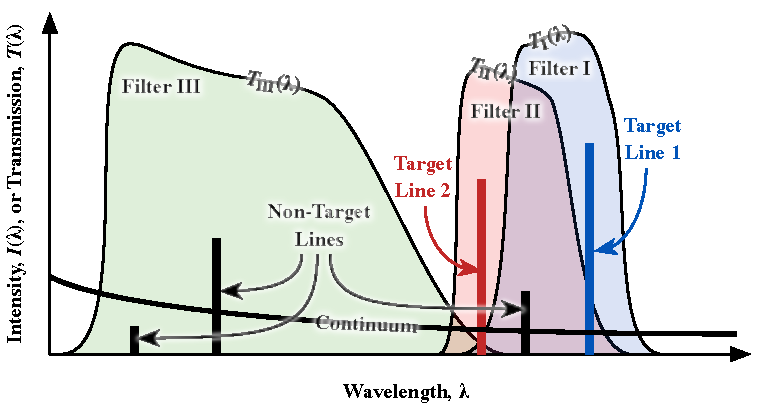
\includegraphics[width=0.8\linewidth]{filter-schematic}
  \caption{Schematic illustration of how the intensity ratio between two target lines is derived using observations in three filters. }
  \label{fig:bandpass}
\end{figure}

We now consider the particular application of deriving a diagnostic
ratio between two emission lines: \(I_1/I_2\).  It is assumed that
observations are made in three filters: Filter~\F{I}, which targets
line~1, Filter~\F{II}, which targets line~2, and Filter~\F{III}, which
targets the continuum.  For optimum results, filters \F{I} and \F{II}
will be narrow-band in order to admit as little continuum as possible,
while \F{III} will be medium-band so as to efficiently sample the
continuum, while at the same time avoiding strong emission lines.
However, in practice it is usually impossible to completely avoid
emission line contamination of filter~\F{III}, either by one or both
of the target lines (1 and 2), or by other lines that we denote
\(i'\).  A schematic illustration of this situation is given in
Figure~\ref{fig:bandpass}.  For given line and continuum intensities,
\(I_1\), \(I_2\), \Icont, the predicted filter rates are:
\begin{align}
  R_{\F{I}} & = \Constant \left[  
    \MeanC{\F{I}}\, \Tmax{\F{I}} W_{\F{I}} 
    + \lambda_1 I_1 \T{1}{\F{I}} + \lambda_2 I_2 \T{2}{\F{I}} 
    + \sum_{i' \ne 1, 2} \lambda_{i'} I_{i'} \T{i'}{\F{I}}
  \right] \label{eq:RI}\\
  R_{\F{II}} & = \Constant \left[  
    \MeanC{\F{II}}\, \Tmax{\F{II}} W_{\F{II}} 
    + \lambda_1 I_1 \T{1}{\F{II}} + \lambda_2 I_2 \T{2}{\F{II}}
    + \sum_{i' \ne 1, 2} \lambda_{i'} I_{i'} \T{i'}{\F{II}}
  \right] \label{eq:RII}\\
  R_{\F{III}} & = \Constant \left[ 
    \MeanC{\F{III}}\, \Tmax{\F{III}} W_{\F{III}} 
    + \lambda_1 I_1 \T{1}{\F{III}}
    + \lambda_2 I_2 \T{2}{\F{III}}
    + \sum_{i' \ne 1, 2} \lambda_{i'} I_{i'} \T{i'}{\F{III}}
   \right] \label{eq:RIII}
\end{align}
% Note that these equations do not describe the most general case, since
% they assume that there is negligible contamination of the narrow-band
% filters by the ``other'' target line, such that \(\T{1}{\F{II}} =
% \T{2}{\F{I}} = 0\).\footnote{This is a good approximation for the line
%   ratios studied in this paper, but in other cases cannot always be
%   assumed.  The general case, which is rather more cumbersome, is
%   treated in \citet{Henney:Calibration}.}  
The mean continuum intensity in the narrow filters can be related to
that in the wider filter by defining color terms: 
\begin{equation}
  \label{eq:color}
  \Color{j}{\F{III}} \equiv \frac{\MeanC{j}}{\MeanC{\F{III}}} \quad
  \text{for \(j =\) \F{I}, \F{II}}
\end{equation}
The filter color terms can be formally extended to include the
contribution of contaminating non-target emission lines:
\begin{equation}
  \label{eq:color-twiddle}
  \COLOR{j}{\F{III}} \equiv 
  \frac{\MeanC{j} + (\Tmax{j} W_j)^{-1} \sum_{\scriptscriptstyle i' \ne 1, 2} \lambda_{i'} I_{i'} \T{i'}{j}}
  {\MeanC{\F{III}} + (\Tmax{\F{III}} W_{\F{III}})^{-1} \sum_{\scriptscriptstyle i' \ne 1, 2} \lambda_{i'} I_{i'} \T{i'}{\F{III}}}
= 
\frac{\left(1 + \sum_{\scriptscriptstyle i' \ne 1, 2} E_{i'} / \Weff{j}{i'}\right) \, \Color{j}{\F{III}} }
{1 + \sum_{\scriptscriptstyle i' \ne 1, 2} E_{i'} / \Weff{\F{III}}{i'}}
\end{equation}
where the \(E_{i'}\) are the equivalent width (in \AA) of each
non-target line and we have also introduced an ``effective width'' of
each filter with respect to a given emission line:
\begin{equation}
  \label{eq:effective}
  \Weff{j}{i} \equiv \Color{j}{i} \frac{\Tmax{j}}{\T{i}{j}} W_j 
  \quad \text{with} \quad
  \Color{j}{i} \equiv \frac{\MeanC{j}}{\lambda_i I_\lambda^i} . 
\end{equation}
Note that the effective width has the property that \(\Weff{j}{i}
\simeq W_j \) for lines \(i\) that lie comfortably within the bandpass
of filter \(j\), whereas \(\Weff{j}{i} > W_j \) for lines that lie
on the edge of the bandpass, where the filter transmission is reduced,
and \(\Weff{j}{i} \to \infty \) for lines far-removed from the filter
bandpass. 

\begin{table}[t]
  \caption{Filter contamination coefficients, see eq.~(\ref{eq:solve-ratio})}
  \label{tab:coefficients}
  \small
  \medskip
  \begin{tabular}{llrrrrrr}\toprule
    Ratio: \(I_1/I_2\)& Filter Set: \F{I}, \F{II}, \F{III} & 
    \(\Falpha{1}\) &
    \(\Falpha{2}\) & 
    \(\Fbeta{I} \) &
    \(\Fbeta{II}\) &
    \(\Fgamma{1} \) &
    \(\Fgamma{2}\) \\
    \midrule
    \nii{} 5755/6583 & FQ575N, F658N, F547M & 
    0.845 & \(\sim 0\) & 0.0243 & 0.0394 & \(\sim 0\) & \(\sim 0\) \\
    \sii{} 6716/6731 & FQ672N, FQ674N, F673N &
    0.994 & 1.12 & 0.164 & 0.114 & 0.02586 & 0.005629 \\
    \sii{} 6716/6731 & FQ672N, FQ674N, F547M &
    \(\sim 0\) & \(\sim 0\) & 0.0274 & 0.0191  & 0.02586 & 0.005629 \\ 
    \oiii{} 4363/5007 & FQ437N, F502N, FQ436N &
    0.968 & \(\sim 0\) & 0.711 & 1.998 & \(\sim 0\) & \(\sim 0\) \\ 
    \oiii{} 4363/5007 & FQ437N, F502N, F547M &
    \(\sim 0\) & 0.00141 & 0.03426 & 0.09627 & \(\sim 0\) & \(\sim 0\) \\ 
    H\(\beta\)/H\(\alpha\) 4861/6563 & F487N, F656N, F547M &
    \(\sim 0\) & \(\sim 0\) & 0.08711 & 0.02375 & \(\sim 0\) & \(\sim 0\) \\
    \bottomrule
  \end{tabular}
  \par\smallskip Note: Values marked as ``\(\sim 0\)'' are all less than \(10^{-5}\). 
\end{table}

With these definitions, equations~(\ref{eq:RI}) to~(\ref{eq:RIII}) can be recognised as being equivalent to a single matrix equation that gives the vector of count rates, \(\left[   R_{\F{I}}\,;\, R_{\F{II}}\,;\, R_{\F{III}}\right] \), in terms of the vector of intensities, \(\left[ \lambda_1 I_1\,;\, \lambda_2 I_2\,;\, \MeanC{\F{III}}\right]\).  Therefore, in order to solve for the intensities in terms of the count rates it is sufficient to invert the matrix.  The result for the line ratio is then:
\begin{equation}
  \label{eq:solve-ratio}
  \frac{I_1}{I_2} = \frac{\lambda_2 \T{2}{\F{II}}}{\lambda_1 \T{1}{\F{I}}}
  \frac{\left[(1 - \Falpha{2} \Fbeta{II} \COLOR{\F{II}}{\F{III}} ) R_{\F{I}} + (\Falpha{2} \Fbeta{I} \COLOR{\F{I}}{\F{III}} - \Fgamma{2})  R_{\F{II}} + (\Fgamma{2} \Fbeta{II}  \COLOR{\F{II}}{\F{III}}  - \Fbeta{I} \COLOR{\F{I}}{\F{III}}) R_{\F{III}}\right]}
  {\left[(\Falpha{1} \Fbeta{II} \COLOR{\F{II}}{\F{III}} - \Fgamma{1}) R_{\F{I}} + (1 - \Falpha{1} \Fbeta{I} \COLOR{\F{I}}{\F{III}}) R_{\F{II}} + (\Fgamma{1} \Fbeta{I} \COLOR{\F{I}}{\F{III}} - \Fbeta{II} \COLOR{\F{II}}{\F{III}}) R_{\F{III}}\right]}
\end{equation}
with filter contamination coefficients
\begin{displaymath}
  \Falpha{1} = \frac{\T{1}{\F{III}}}{\T{1}{\F{I}}} ; \quad 
  \Falpha{2} = \frac{\T{2}{\F{III}}}{\T{2}{\F{II}}} ; \quad
  \Fbeta{I}  = \frac{\Tmax{\F{I}} W_{\F{I}}}{\Tmax{\F{III}} W_{\F{III}}} ; \quad
  \Fbeta{II}  = \frac{\Tmax{\F{II}} W_{\F{II}}}{\Tmax{\F{III}} W_{\F{III}}} ; \quad
  \Fgamma{1}  = \frac{\T{1}{\F{II}}}{\T{1}{\F{I}}} ; \quad 
  \Fgamma{2}  = \frac{\T{2}{\F{I}}}{\T{2}{\F{II}}} .
\end{displaymath}
The \(\alpha\) contamination coefficents give the throughput of each
target emission line in the continuum filter \F{III} relative to the
throughput in its respective narrow-band filter, and will tend to be
either \(\sim 1\) for lines that fall in the continuum bandpass, or
\(\sim 0\) for those that do not.  The \(\beta\) contamination
coefficients give the integrated continuum throughput in each narrow
band filter relative to the continuum filter.  The \(\gamma\)
contamination coefficients give the throughput of each target emission
line in the ``other'' narrow band filter relative to the throughput in
its own narrow-band filter, and will only be important in cases where
the two narrow band filters overlap.

Since repeated
calibration programs have shown that the WFC3 filter characteristics
are stable with time, all these purely instrumental coefficients are
constants, albeit with a small systematic uncertainty in their true value.
The \(\widetilde{k}\) factors, on the other hand, represent the
relative strengths of the continuum and non-target lines in the
bandpasses of the three filters, and are expected to show variations
from object to object and from pixel to pixel within the same object,
due to changes in the physical conditions. 

\begin{figure}
  \centering
  \begin{tabular}{ll}
    (\textit{a}) & (\textit{b}) \\
    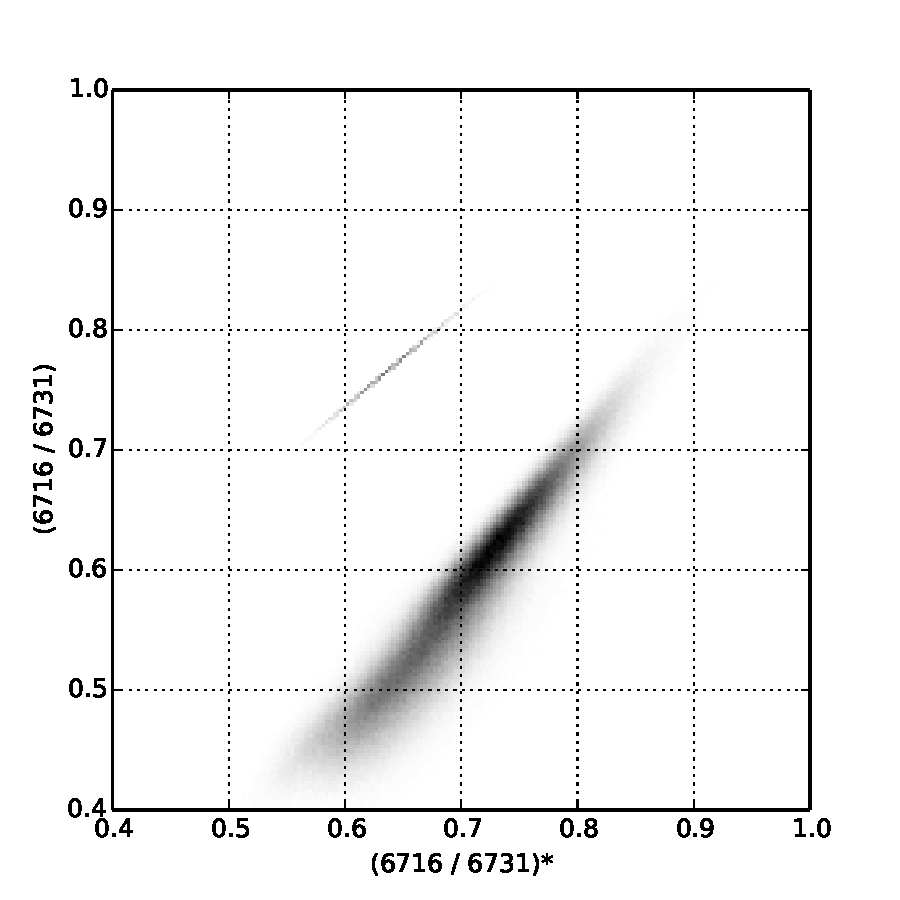
\includegraphics[width=0.45\linewidth]{contam-correct-FQ672N-FQ674N-F673N}
    &
    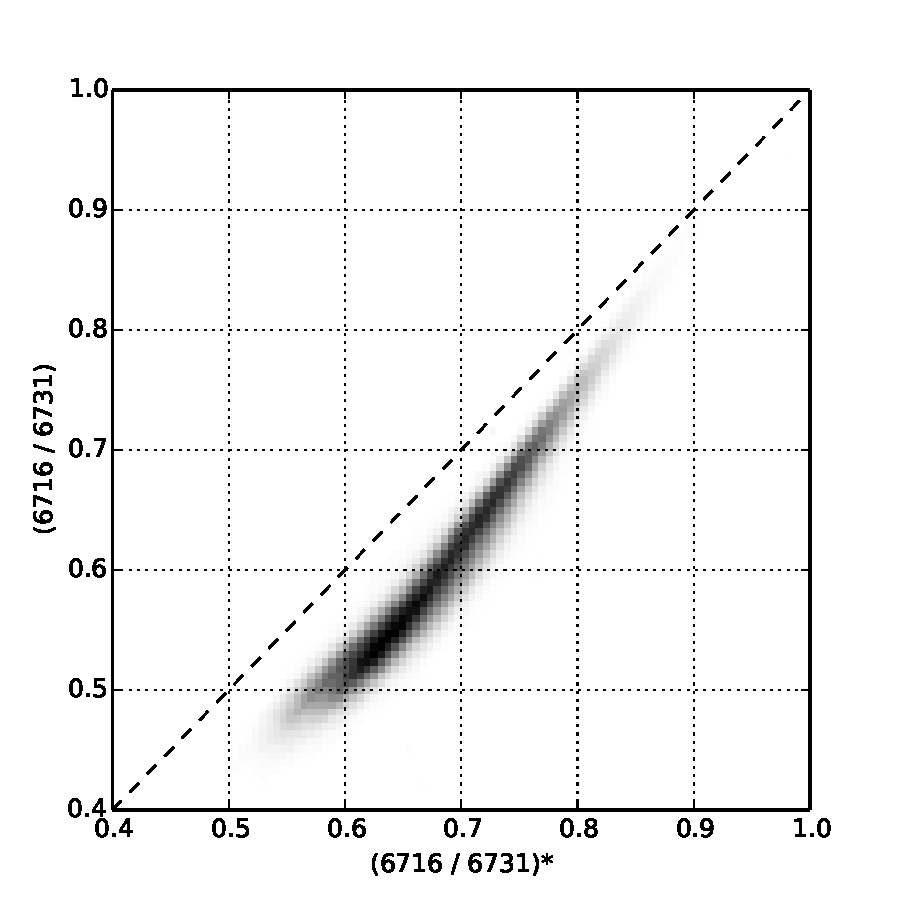
\includegraphics[width=0.45\linewidth]{contam-correct-FQ672N-FQ674N-F547M} \\
    (\textit{c}) & (\textit{d}) \\
    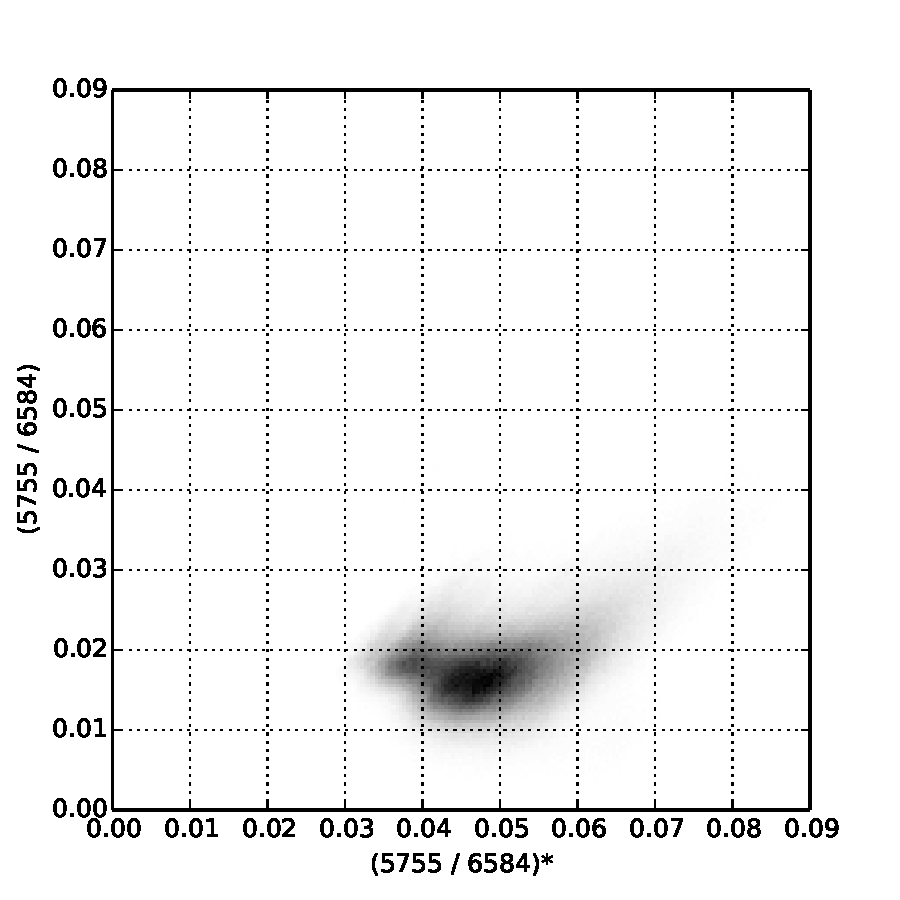
\includegraphics[width=0.45\linewidth]{contam-correct-FQ575N-F658N-F547M}
    &
    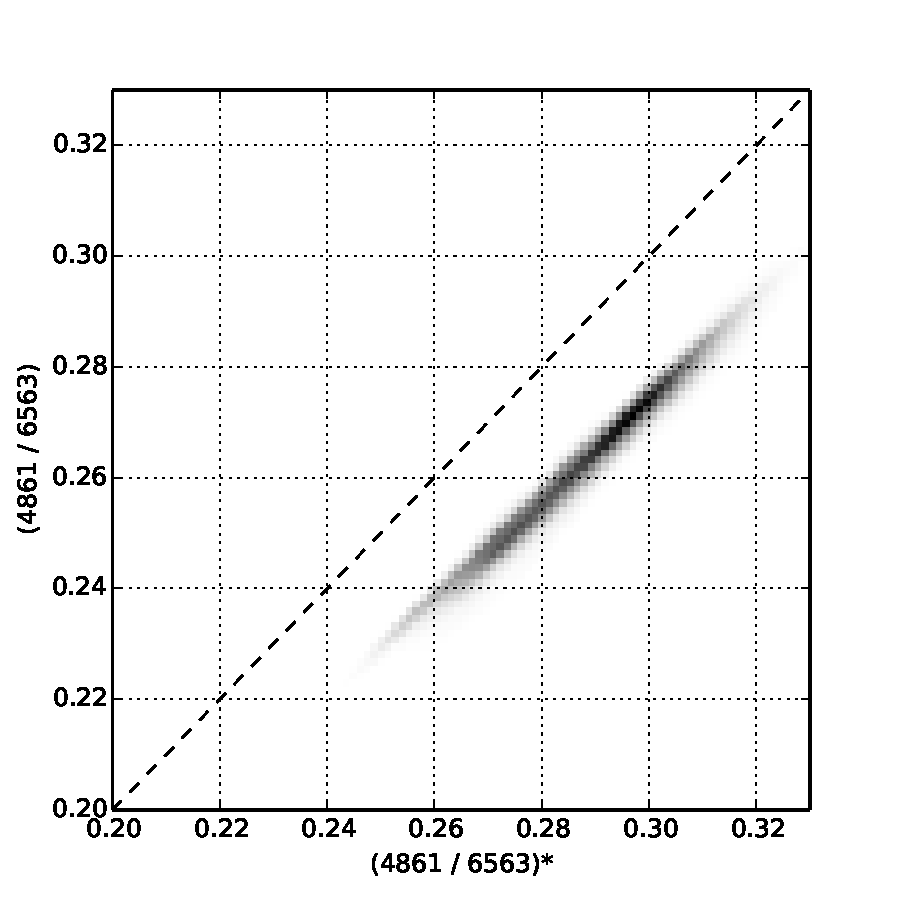
\includegraphics[width=0.45\linewidth]{contam-correct-F487N-F656N-F547M}
  \end{tabular}
  \caption{Effects on derived line ratios of contamination by
    continuum and non-target lines.  In each panel, the \(x\) axis
    shows the ``naive'' line ratio, while the \(y\) axis shows the
    corrected line ratio.  (\textit{a})~\sii{} 6716/6731 ratio
    caclulated from FQ672N, FQ674N, F673N; (\textit{b})~\sii{} 6716/6731 ratio
    caclulated from FQ672N, FQ674N, F547M; (\textit{c})~\nii{} 5755/6583 ratio
    caclulated from  FQ575N, F658N, F547M;
    (\textit{d})~H\(\beta\)/H\(\alpha\) ratio calculated from F487N,
    F656N, F547M.}
  \label{fig:contam}
\end{figure}

\begin{figure}
  \centering
  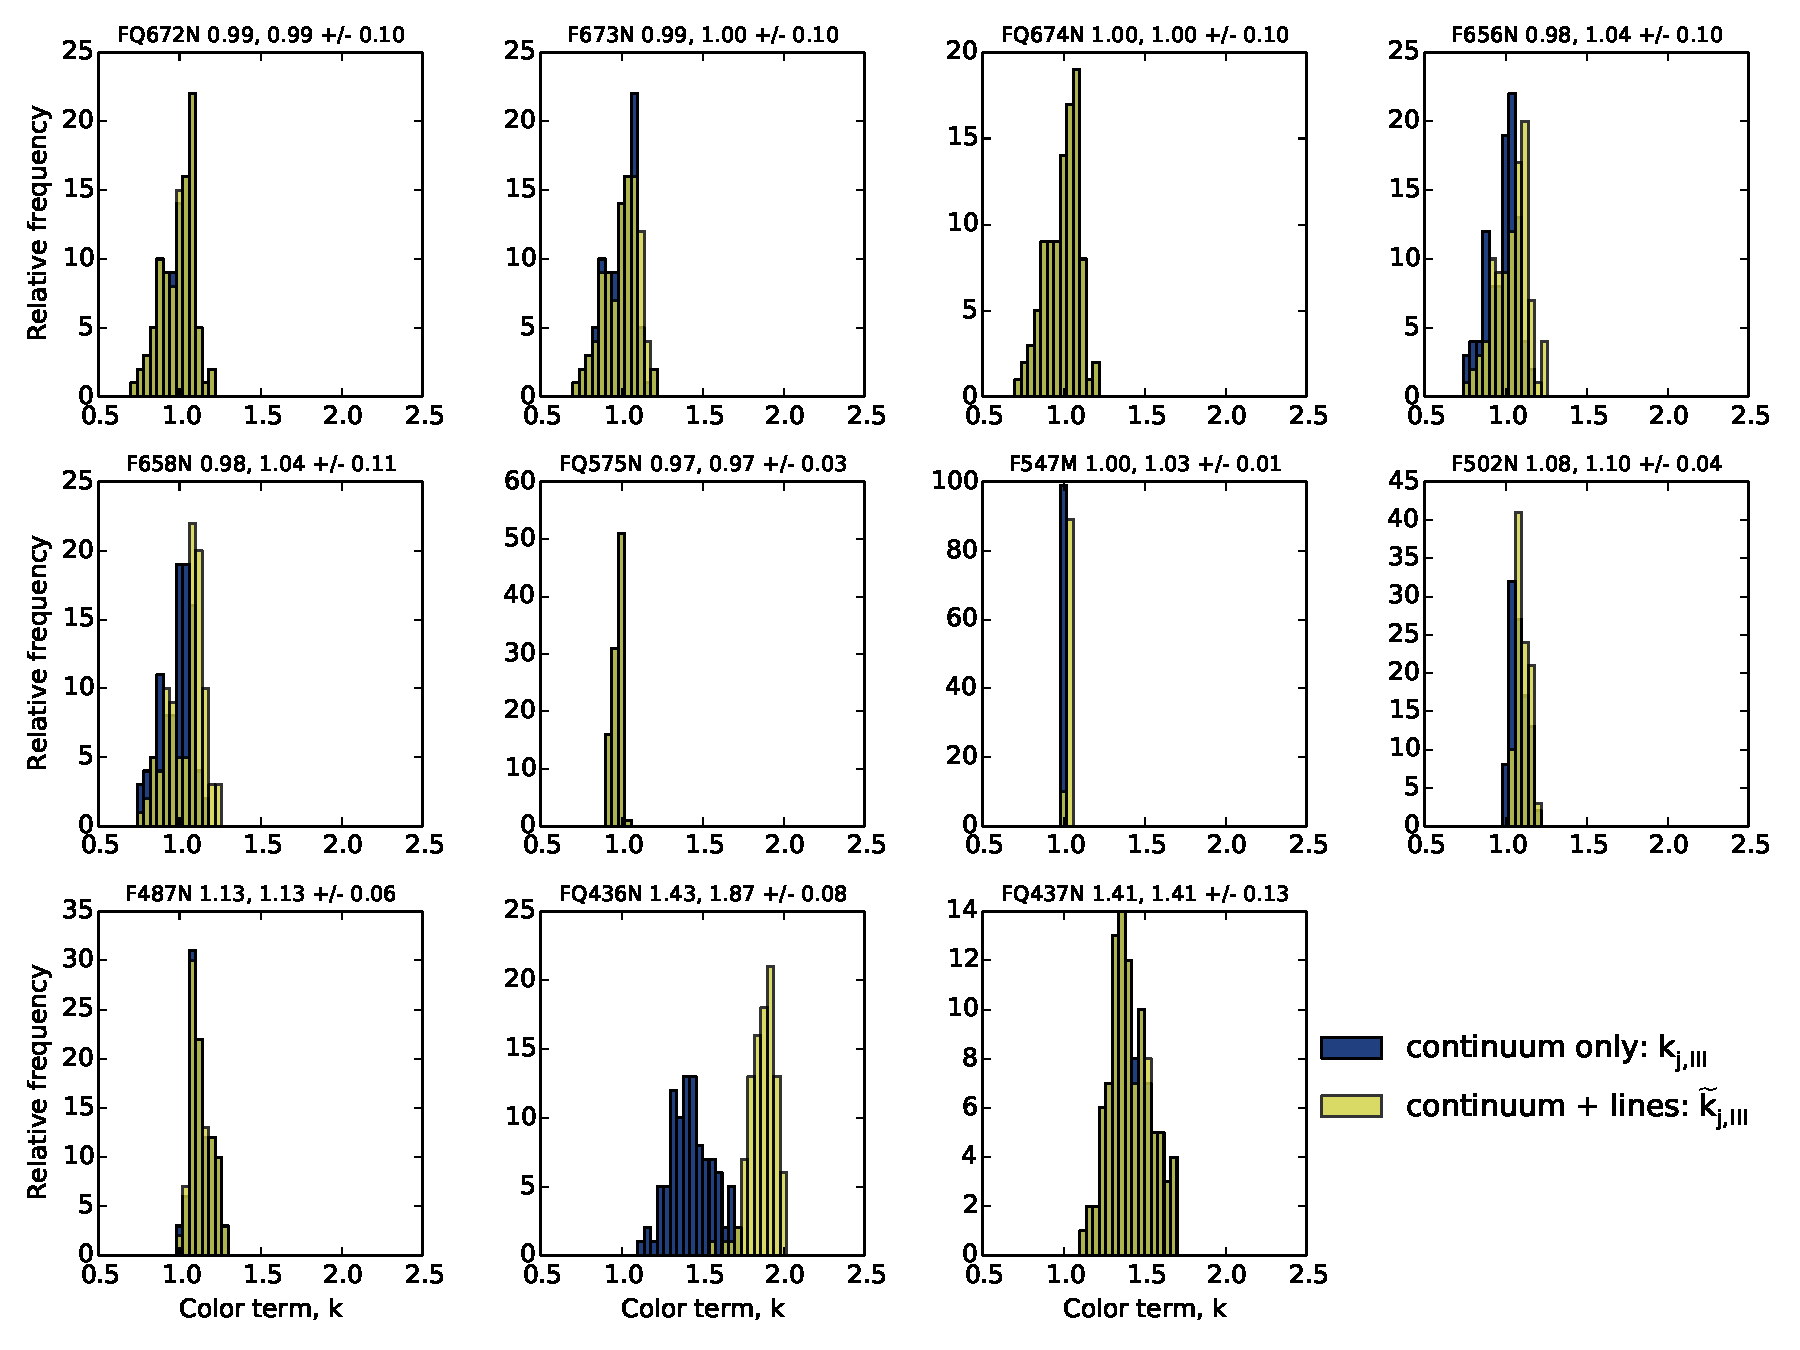
\includegraphics[width=\linewidth]{odh-k-color-histograms}
  \caption{Observationally determined histograms of the color
    correction terms, \(k\), for each filter with respect to the F547M
    filter, measured from spectrophotometry of the Orion Nebula
    \citep{ODell:2010a}.  The blue histograms show the ratio of the
    mean continuum intensity in each filter to that in F547M, as given
    by equation~(\ref{eq:color}), while the yellow histograms include
    the additional effect of non-target emission lines and correspond
    to the numerator of fraction on the RHS of
    equation~(\ref{eq:color-twiddle}), except for F547M where they
    correspond to the denominator of that fraction. }
  \label{fig:color-correction}
\end{figure}

\begin{figure}
  \centering
  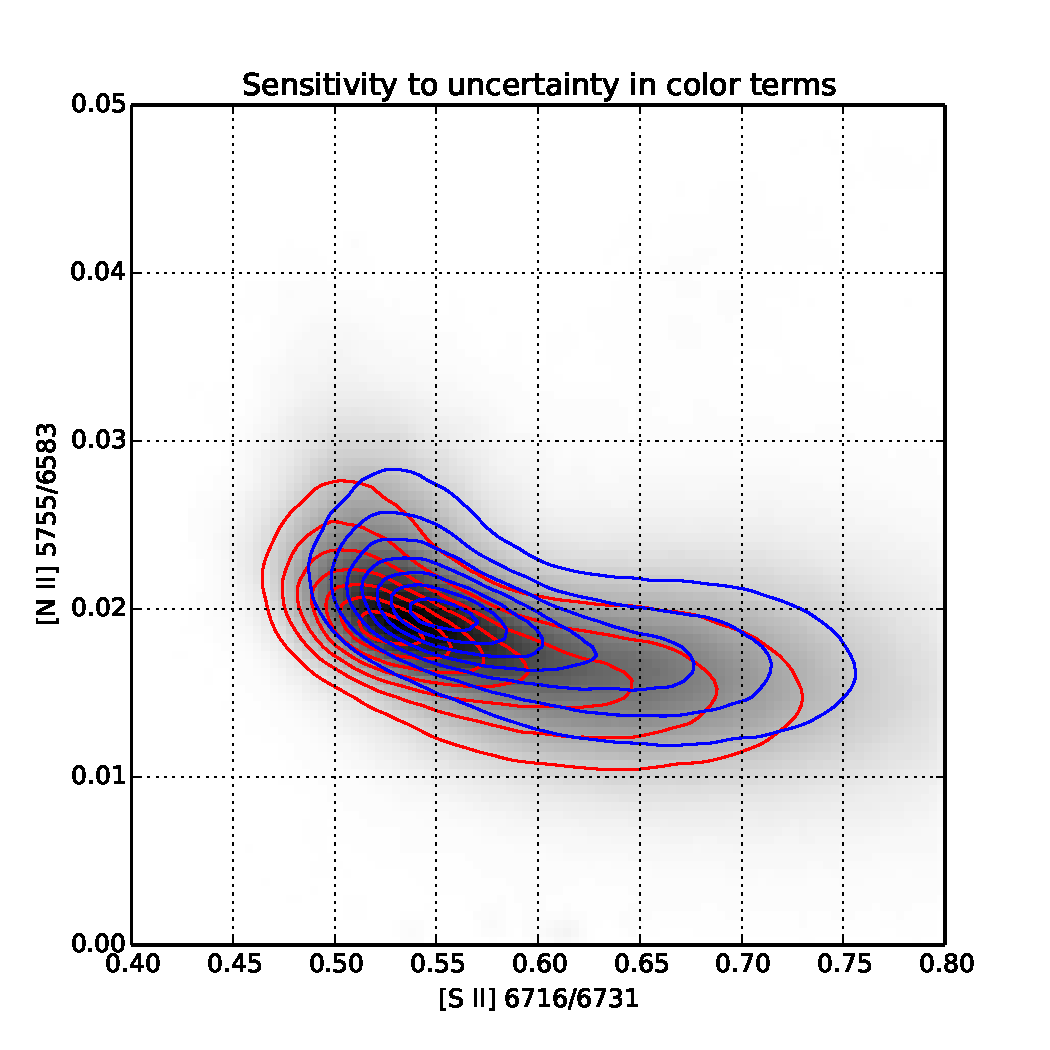
\includegraphics[width=\linewidth]{ratio-sensitivity-ktwiddle}
  \caption{Sensitivity of the derived line ratios to spatial
    variations in the color correction terms.}
  \label{fig:sens-ktwid}
\end{figure}

\begin{figure}
  \centering
  \setlength\tabcolsep{0pt}
  \setkeys{Gin}{width=0.45\linewidth}
  \begin{tabular}{ll}
    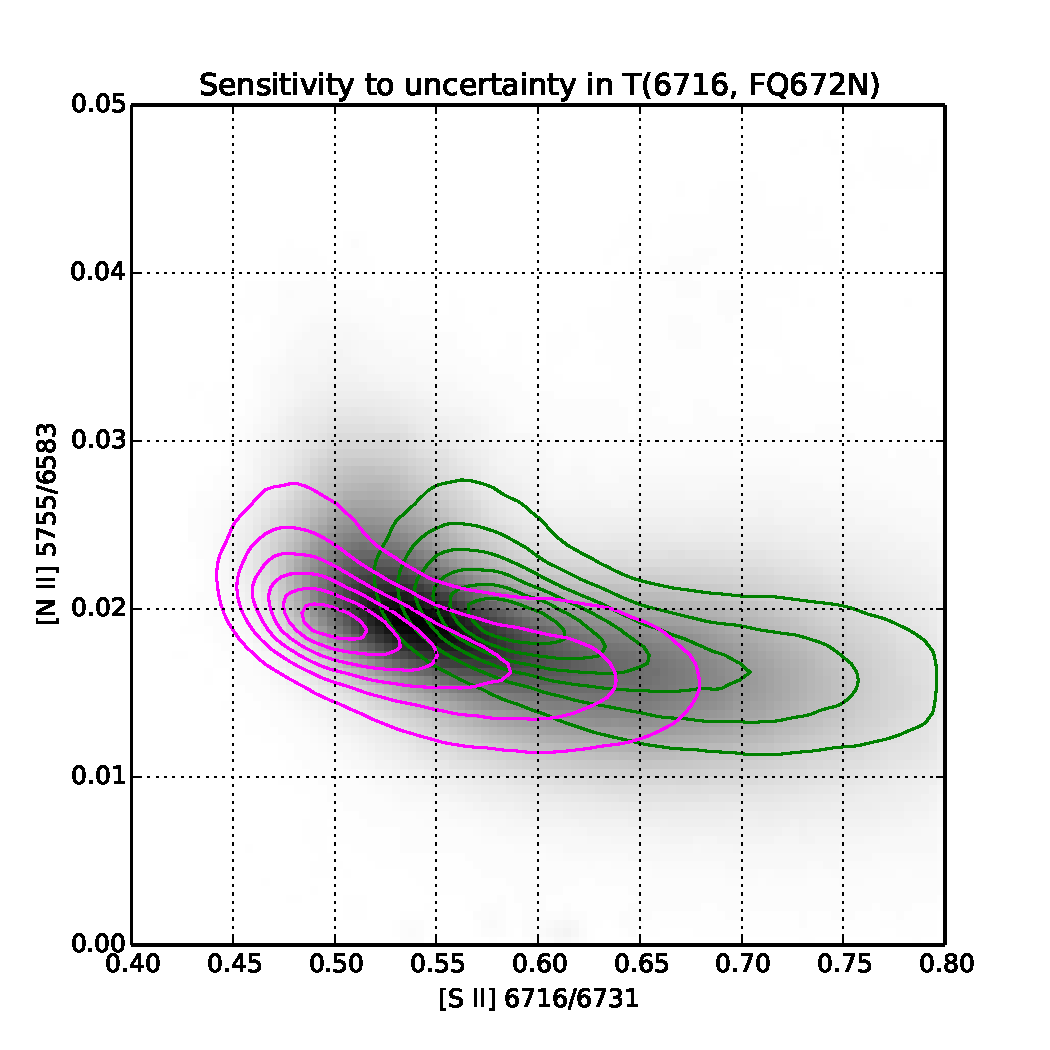
\includegraphics{ratio-sensitivity-T6716-FQ672N} &
    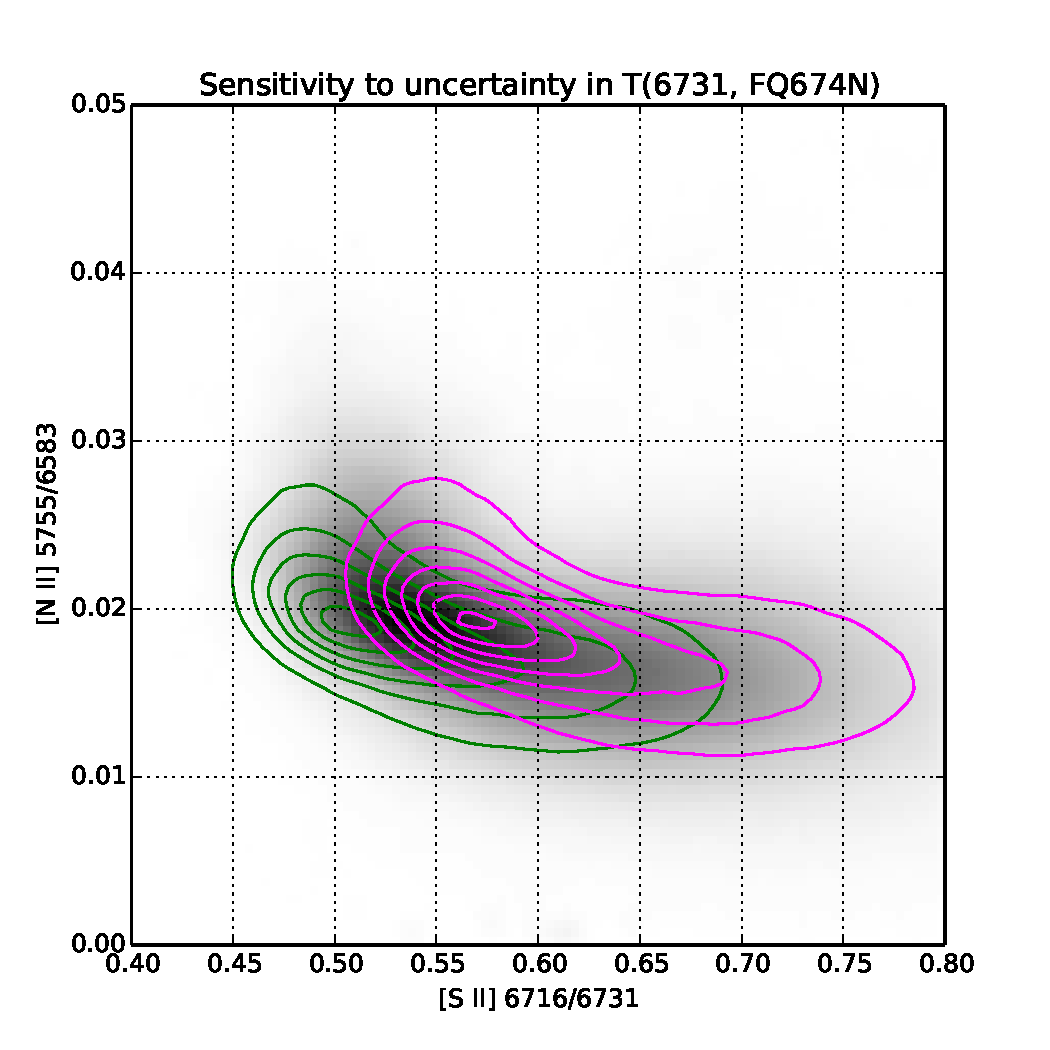
\includegraphics{ratio-sensitivity-T6731-FQ674N} \\
    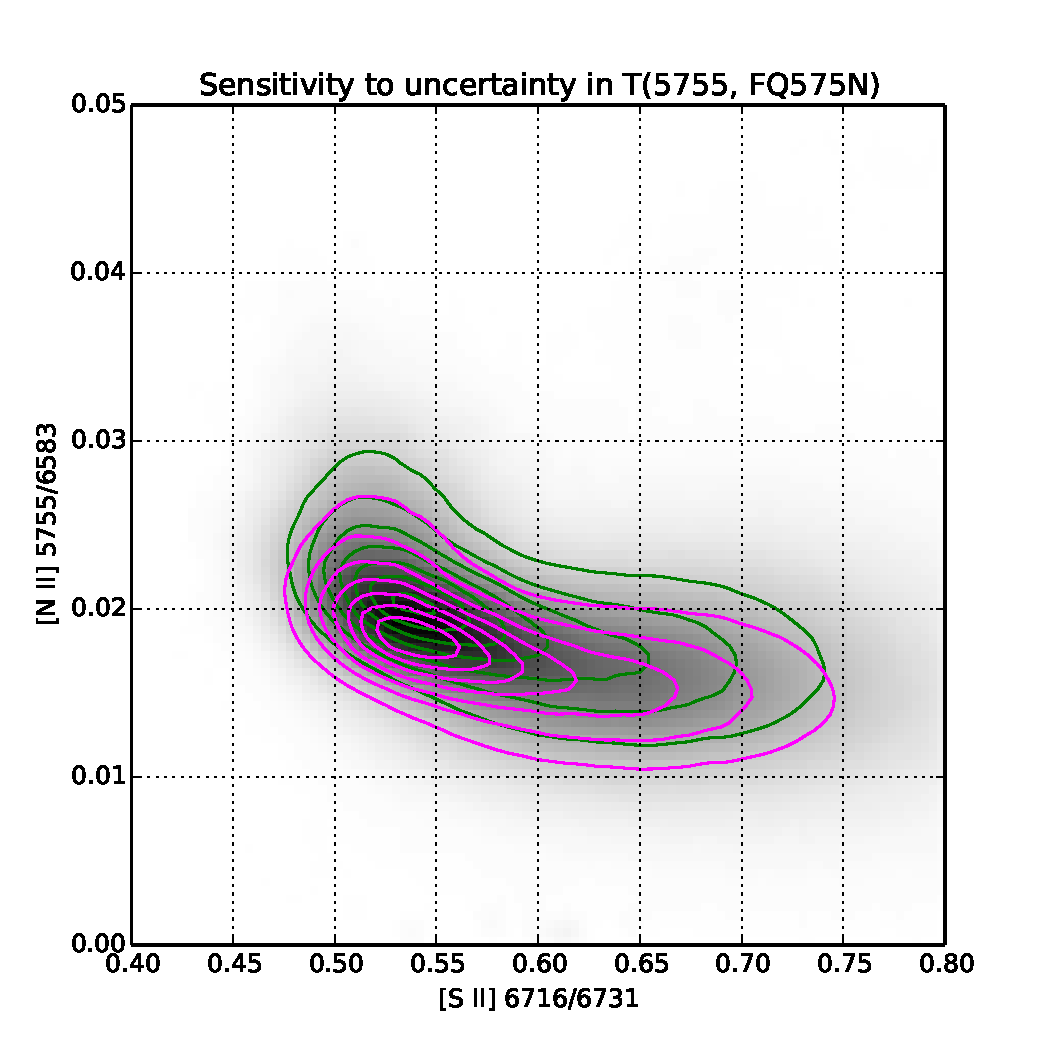
\includegraphics{ratio-sensitivity-T5755-FQ575N} &
    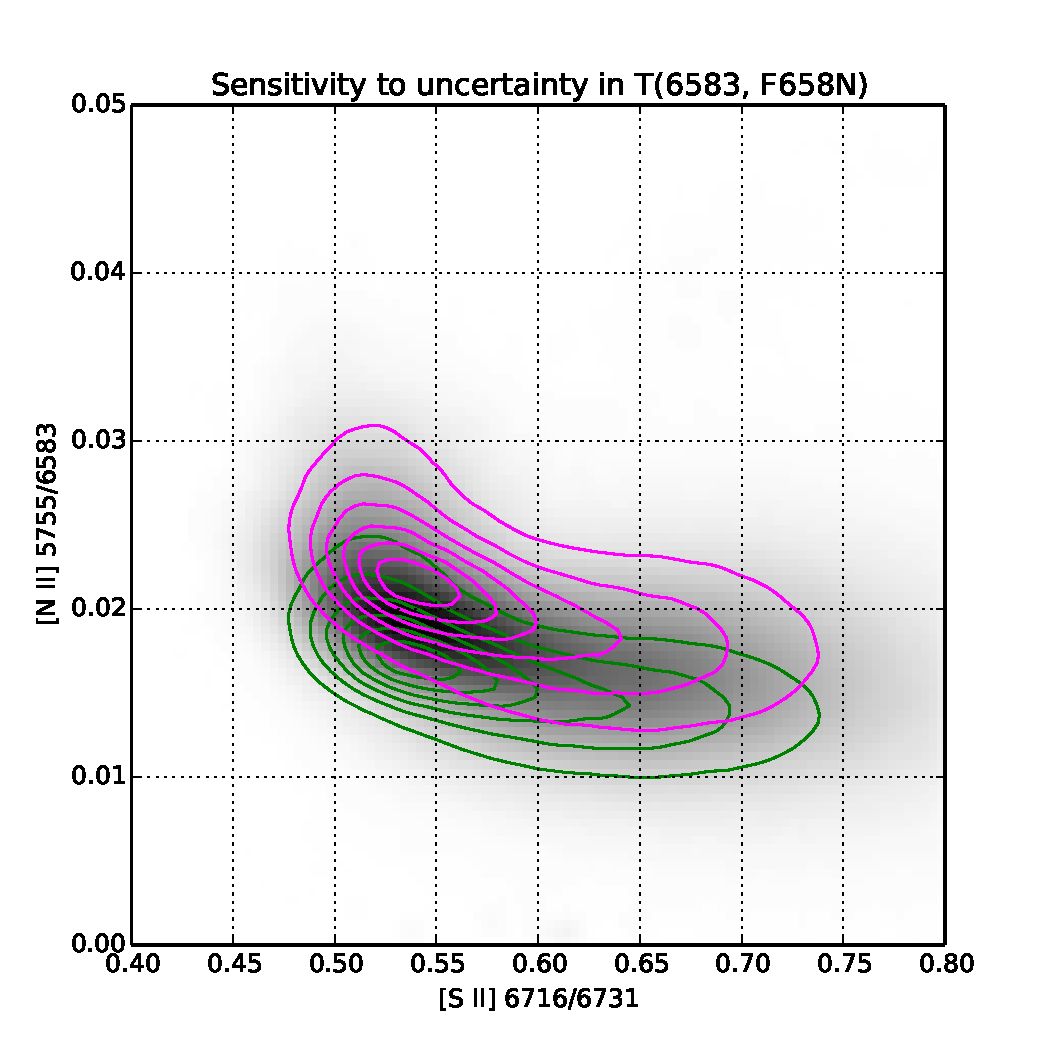
\includegraphics{ratio-sensitivity-T6583-F658N} \\
    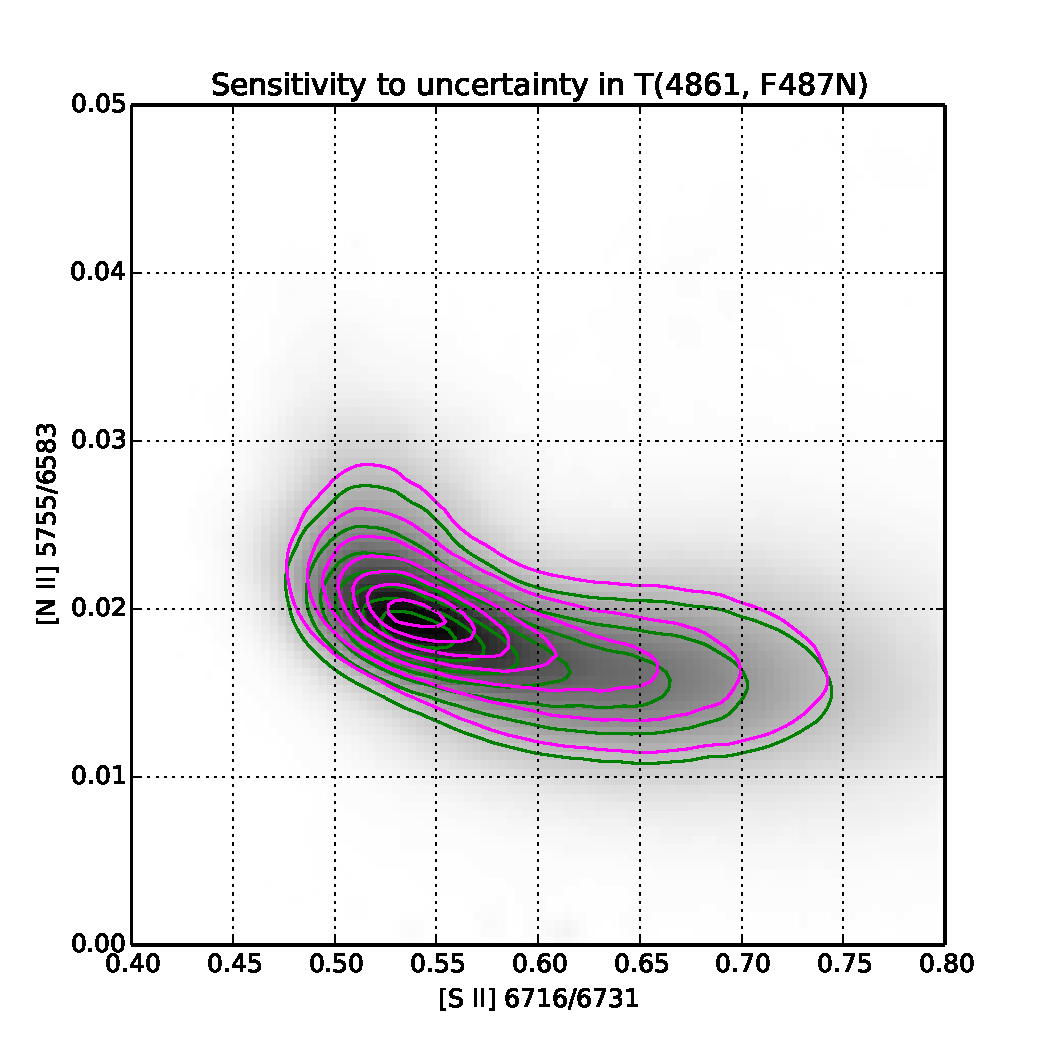
\includegraphics{ratio-sensitivity-T4861-F487N} &
    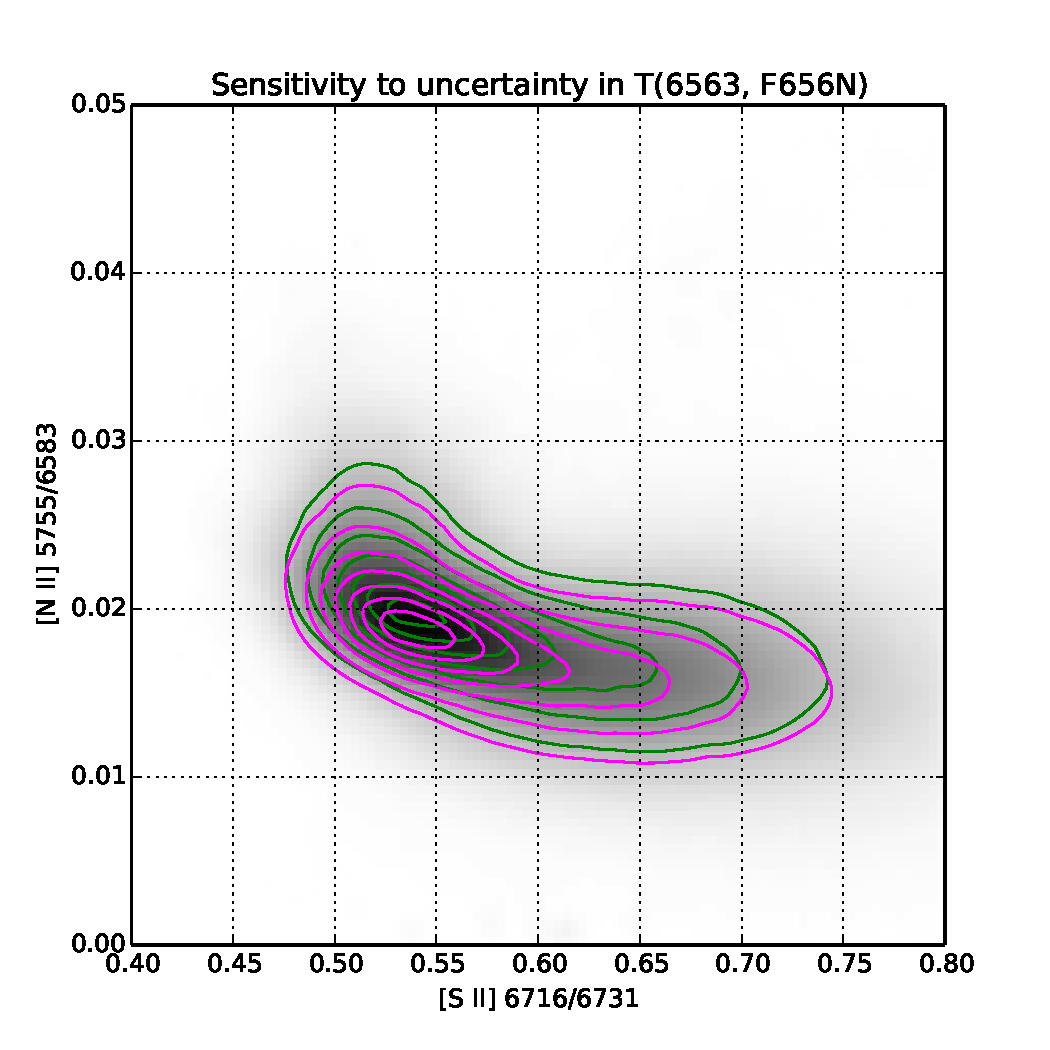
\includegraphics{ratio-sensitivity-T6563-F656N} \\
  \end{tabular}
  \caption{Sensitivity of the derived line ratios to systematic
    uncertainties in the emission line filter throughputs.}
  \label{fig:sens-T}
\end{figure}



\subsection{\boldmath Deriving \(\Te, \Ne\) from line ratios}
\label{sec:derive}

Figure~\ref{fig:deredden} compares our line ratios with selected
measurements from the literature and with the predictions of one-zone
emission models with a unique temperature and density.  Agreement with
previous measurements is good in the bright regions (left of the
diagram), but we deviate from Mesa-Delgado for the fainter regions.
Part of the increase in 5755/6583 to the left of the diagram is due to
higher densities, but there is evidence for an additional temperature
increase over and above that.

However, as can be seen from Figure~\ref{fig:two-phase}, a model with
two different density components along the line of sight can also
explain the top-left of the diagram.  The particular model shown has
two components of equal temperature (\(10,000\)~K), each with the same
emission measure: \(\int n_{\mathrm{e}} n(\mathrm{N^+}) \, dz\).  Over
a wide range of parameter space, the \sii{} ratio is only sensitive to
the density of the lower-density component, while the \nii{} ratio is
only sensitive to the density of the higher-density component.  A
density contrast of a factor of 20 (\(10^4~\mathrm{cm^{-3}}\) and
\(2 \times 10^5~\mathrm{cm^{-3}}\)) is sufficient to mimic a temperature
increase of \(3000\)~K.\@   If this compression were due to a
radiative shock, then it would need a Mach number of \(\sqrt{20}
\simeq 4.5\), corresponding to a velocity of \(50~\mathrm{km\
  s^{-1}}\), which is typical of the jets observed in Orion. 

Although the bi-density mechanism can explain small knots and
filaments with elevated 5755/6583, it cannot readily explain the
general increase in the ratio over a \(10'' \times 10''\) area, as we
see in Orion~S.\@  A real increase in temperature seems a more likely
explanation.  

\begin{figure}
  \centering
  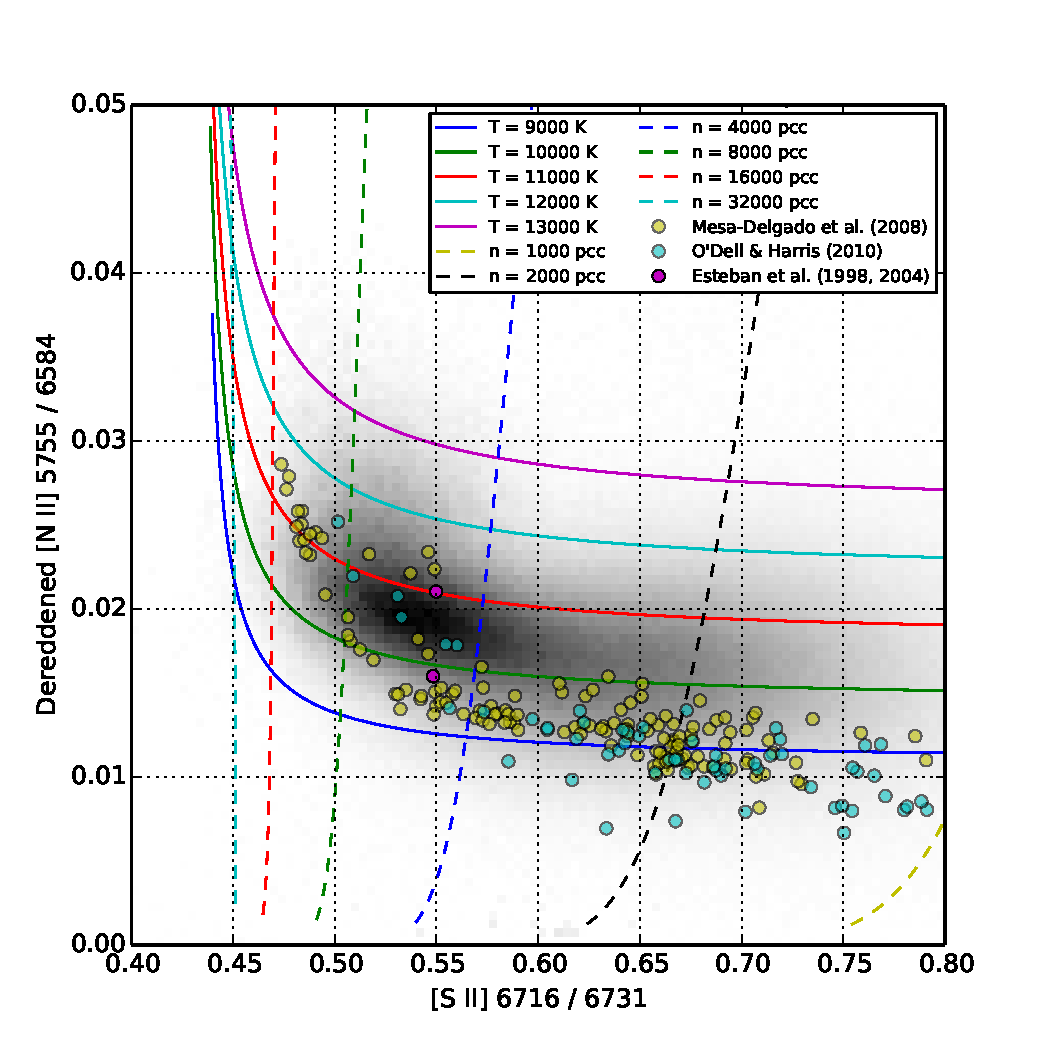
\includegraphics{nii-deredden-vs-sii-ratios}
  \caption{Reddening corrected line ratios for \sii{} and \nii{}}
  \label{fig:deredden}
\end{figure}

\begin{figure}
  \centering
  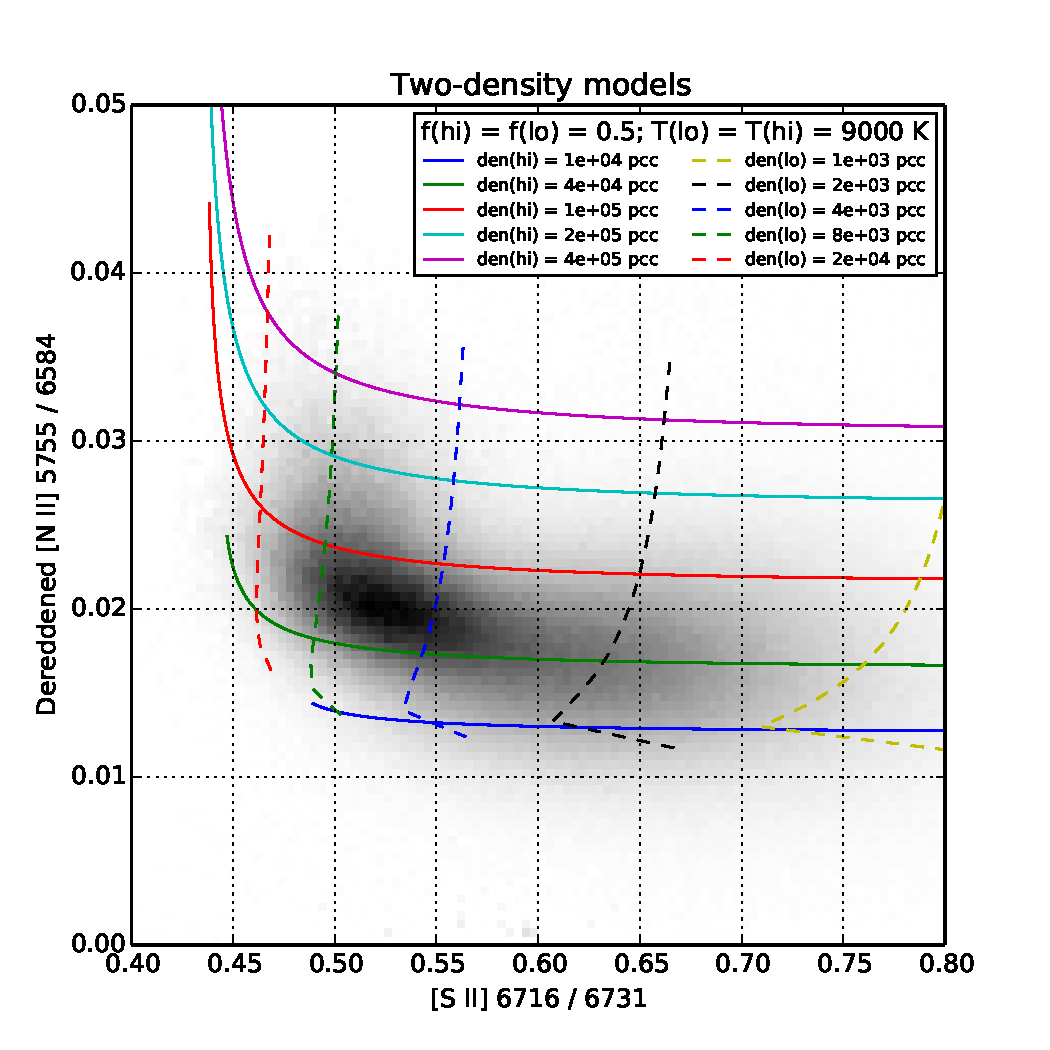
\includegraphics{nii-sii-ratios-two-phase}
  \caption{Same as Fig.~\ref{fig:deredden} but comparing the observed
    ratios with constant-temperature, bi-density models.}
  \label{fig:two-phase}
\end{figure}



\subsection{Strong auroral \nii{} associated with jet filaments}
\label{sec:jets}

See Figures~\ref{fig:rgb-jet} to~\ref{fig:feiii-excess-jet}.  I will
also do another figure that zooms in on the optical outflow source
region.  

Most of the regions with high 5755/6584 ratio are associated with the
bases of stellar outflows. 

Estimate density in HH529 jet from the \ha{} brightness and observed
width.  Compare this with the density required in order to explain the
5755/6583 ratio without invoking higher temperature (see
Fig.~\ref{fig:two-phase}).

\begin{figure}
  \centering
  \includegraphics[width=\linewidth]{jet_region_rgb}
  \caption{Three-color WFC3 image of Orion~S region, immediately to
    the south west of the Trapezium stars, in the light of \sii{}
    6716+31 (F673N; red), \nii{} 6583 (F658N; green) and \oiii{} 5007
    (F502N; blue).  The region shown has a size of \(1.2 \times 0.9\)
    arcminutes.  The filters have not been continuum-subtracted, and
    the F673N filter is the most affected by continuum contamination,
    so all stars show as red, irrespective of their true colors.}
  \label{fig:rgb-jet}
\end{figure}

\begin{figure}
  \centering
  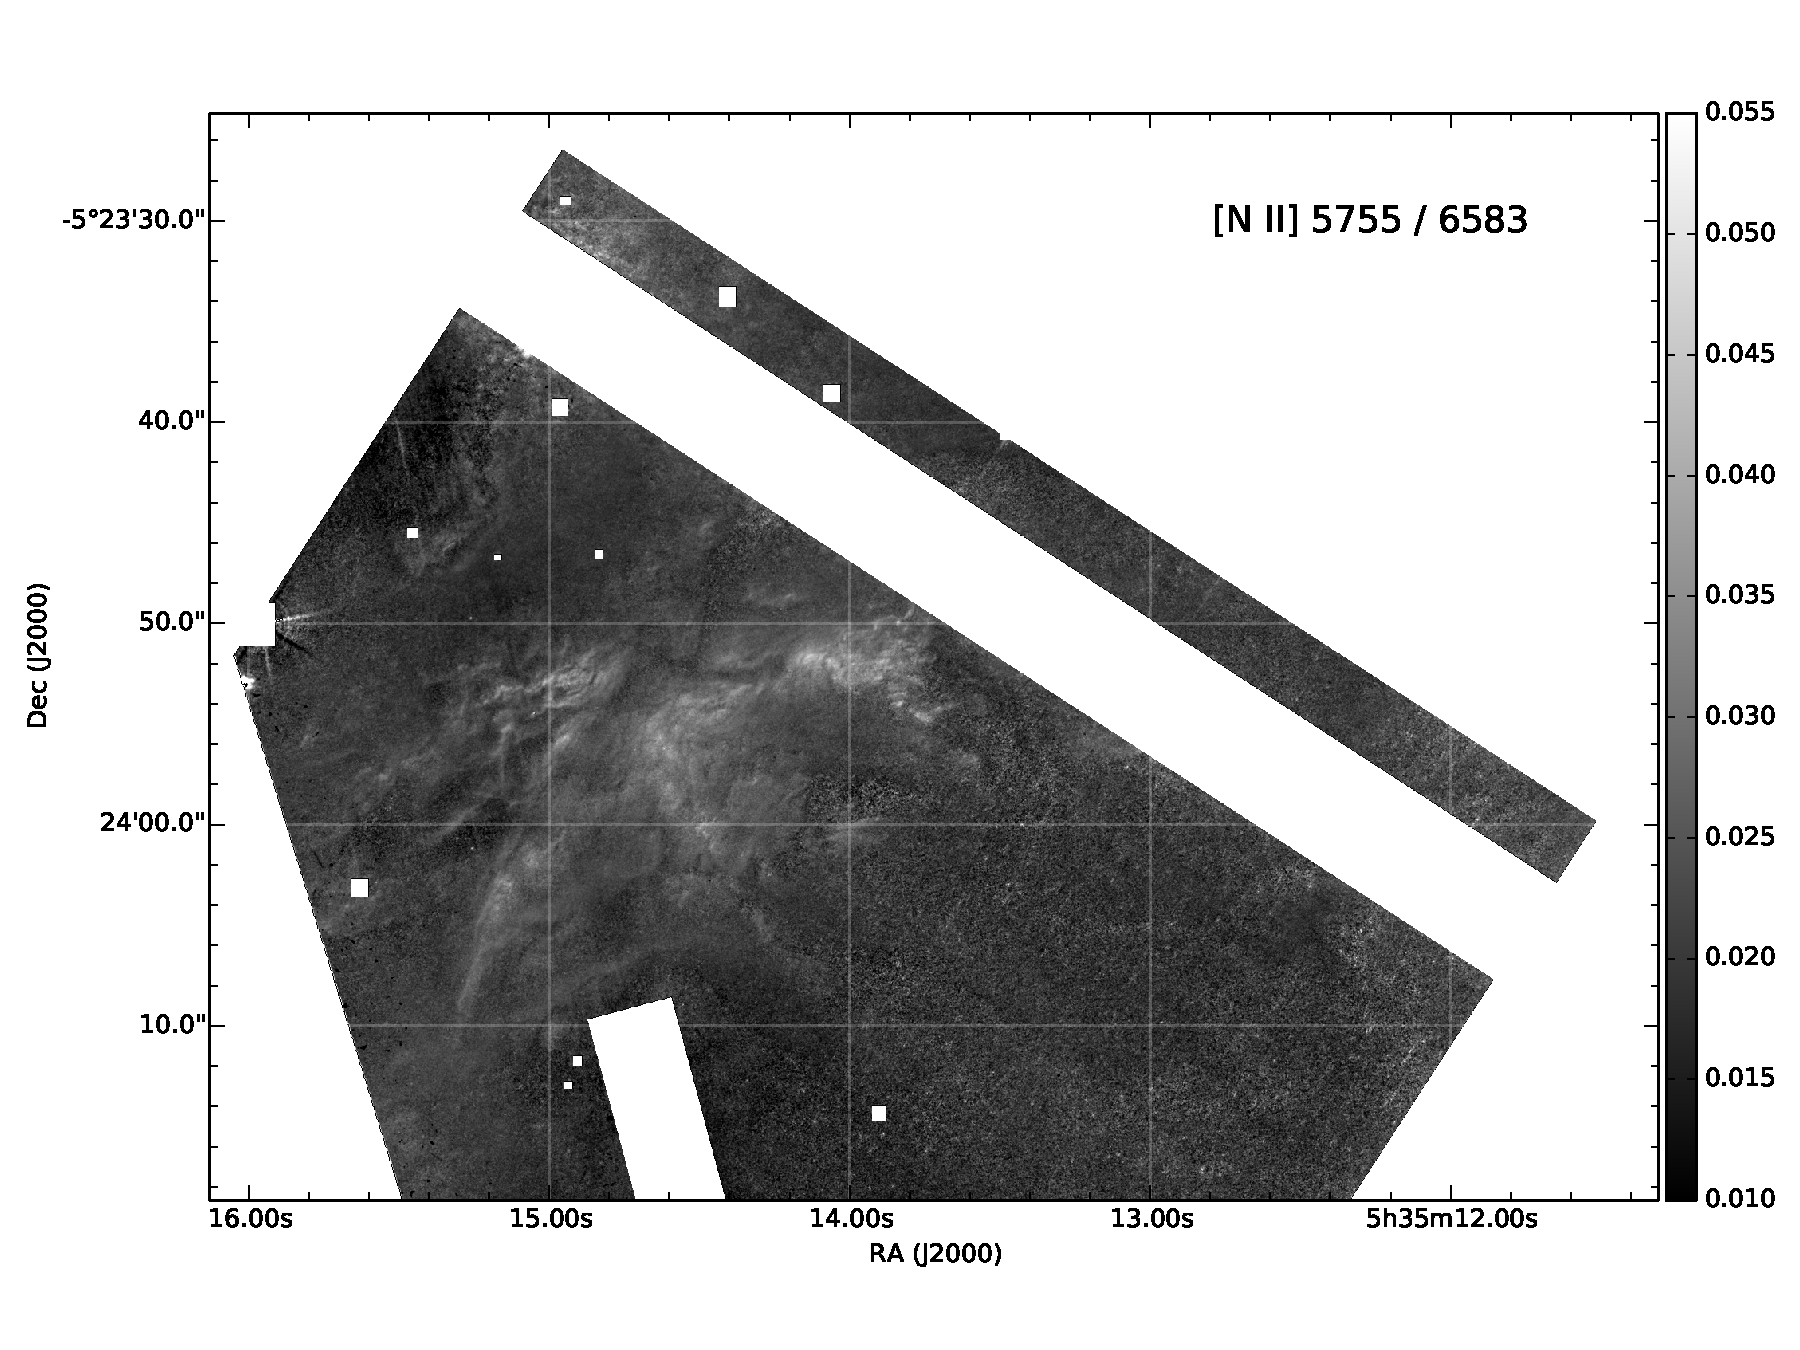
\includegraphics[width=\linewidth]{jet_region_niiratio}
  \caption{Positive grayscale image of the diagnostic \nii{} 5755/6583
    ratio for the same Orion~S region as shown in
    Fig.~\ref{fig:rgb-jet}.  Lighter shades imply higher temperatures
    and/or densities.  The positions of bright stars are masked out in
    the image, as are regions that are badly affected by scattered
    light from the Trapezium stars, which are just outside the fild of
    view.  The ratio is corrected for reddening and calculated
    according to the procedure outlined in \S~\ref{sec:filters}.}
  \label{fig:nii-jet}
\end{figure}

\begin{figure}
  \centering
  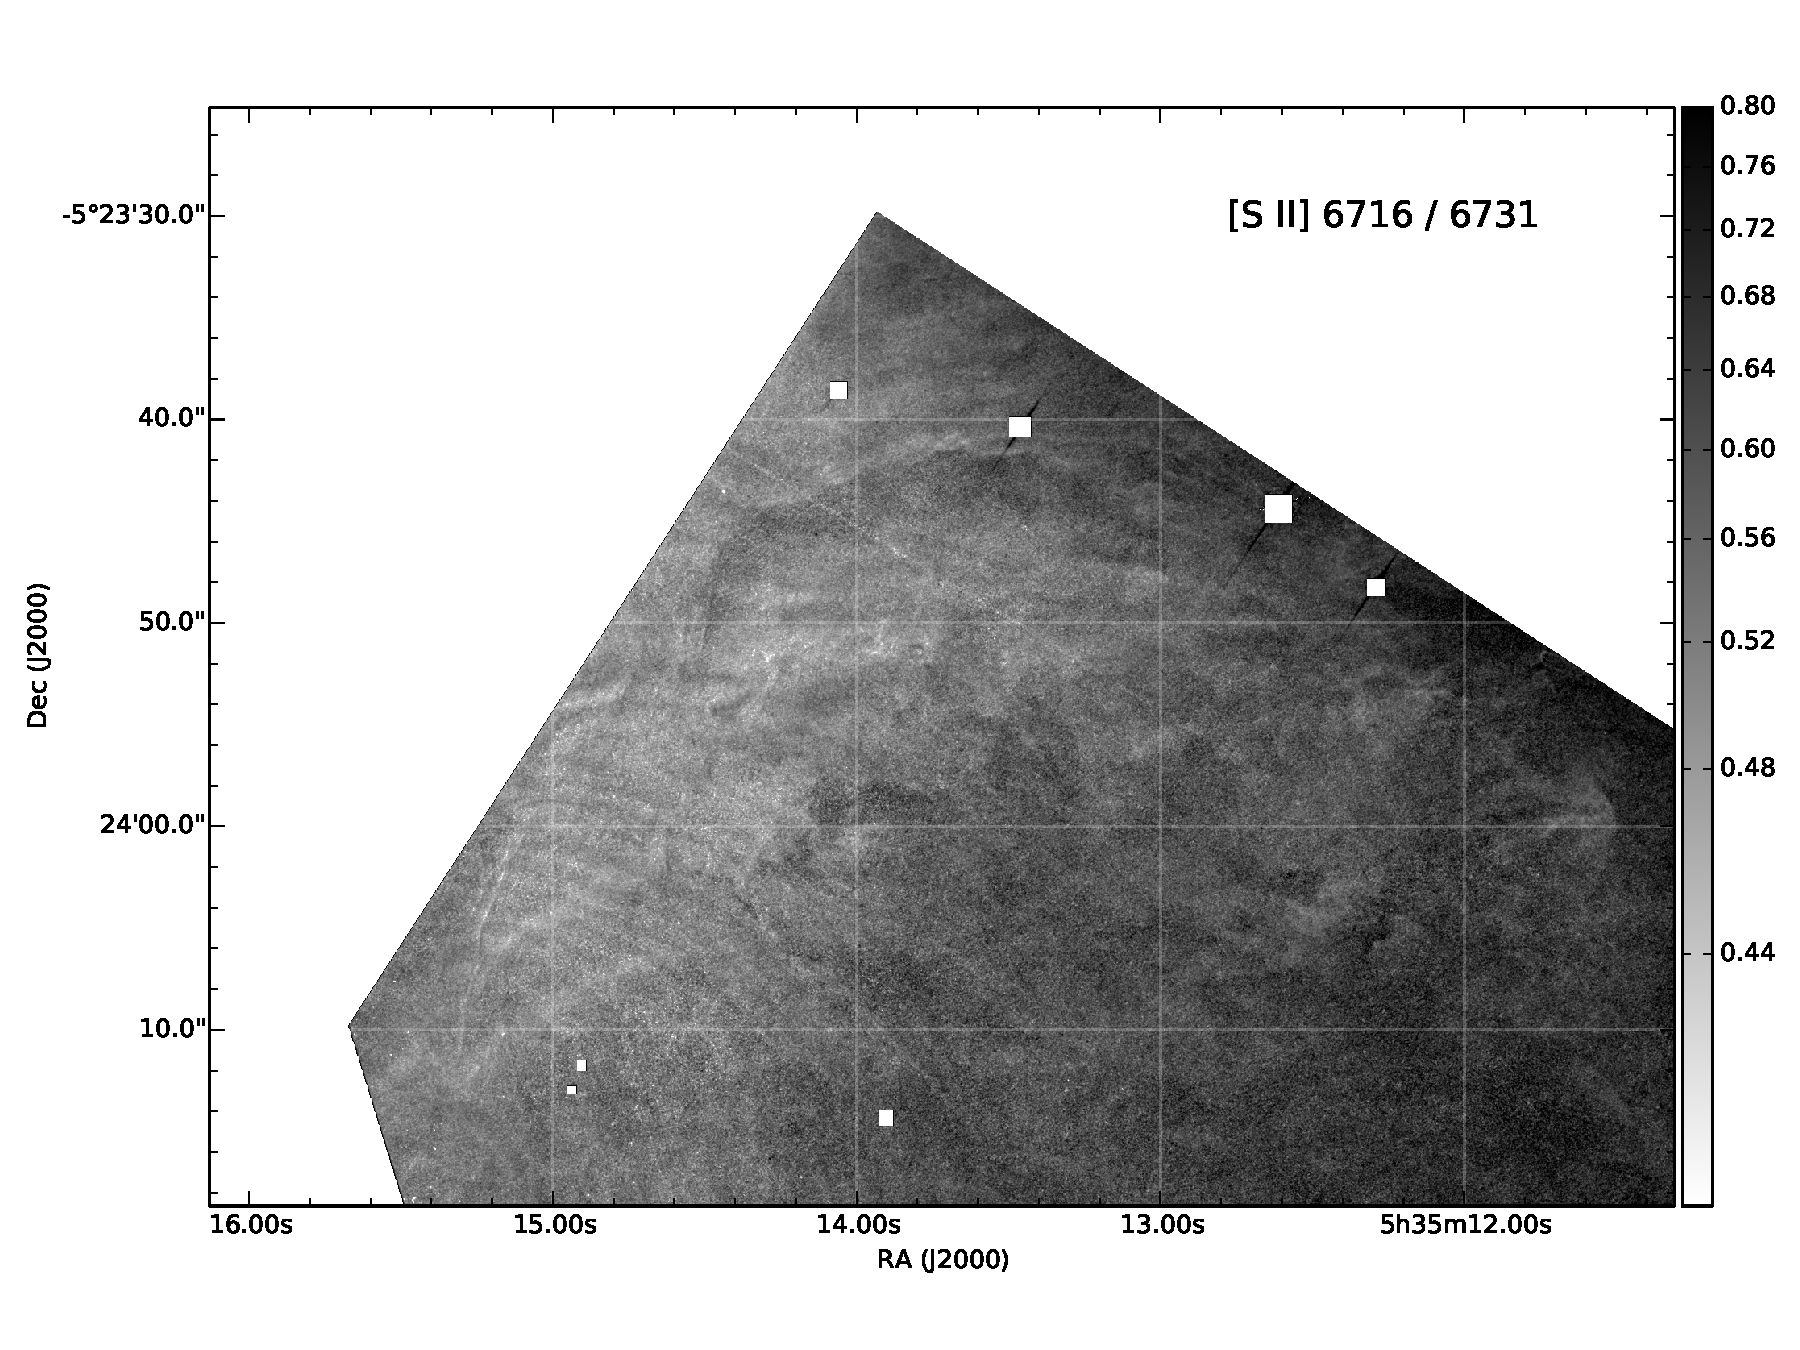
\includegraphics[width=\linewidth]{jet_region_siiratio}
  \caption{Negative grayscale image of the diagnostic \sii{} 6716/6731
    ratio for the same Orion~S region as shown in
    Fig.~\ref{fig:rgb-jet}.  Lighter shades imply higher
    densities.}
  \label{fig:sii-jet}
\end{figure}

\begin{figure}
  \centering
  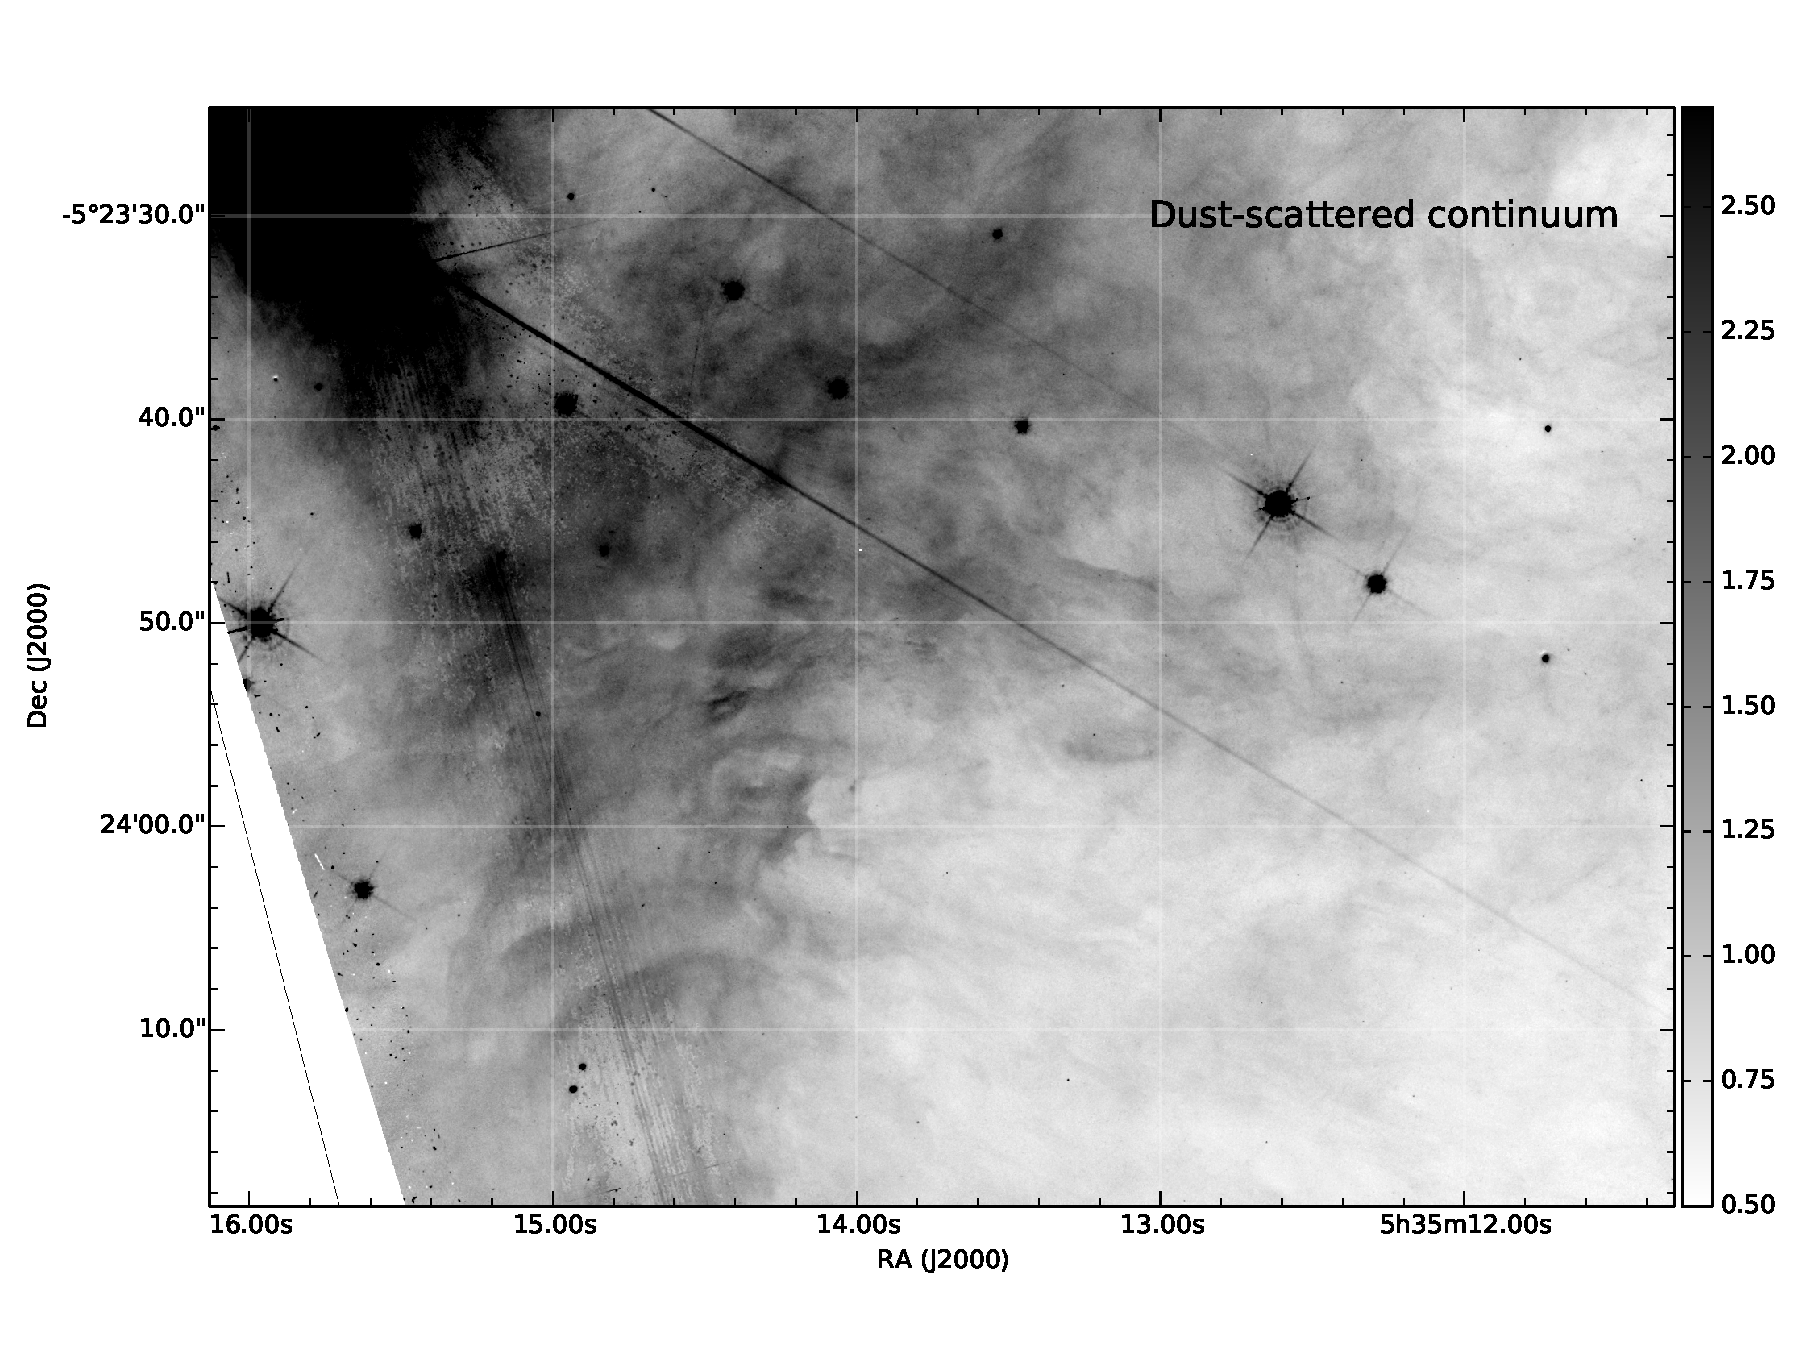
\includegraphics[width=\linewidth]{jet_region_scattered}
  \caption{Negative grayscale image of dust-scattered continuum for
    the same Orion~S region as shown in Fig.~\ref{fig:rgb-jet}.  The
    image was calculated by subtracting an estimate of the atomic
    recombination continuum from the signal in the F547M filter (see
    text for details).  Darker shades correspond to higher surface
    brightness.}
  \label{fig:scatter-jet}
\end{figure}

\begin{figure}
  \centering
  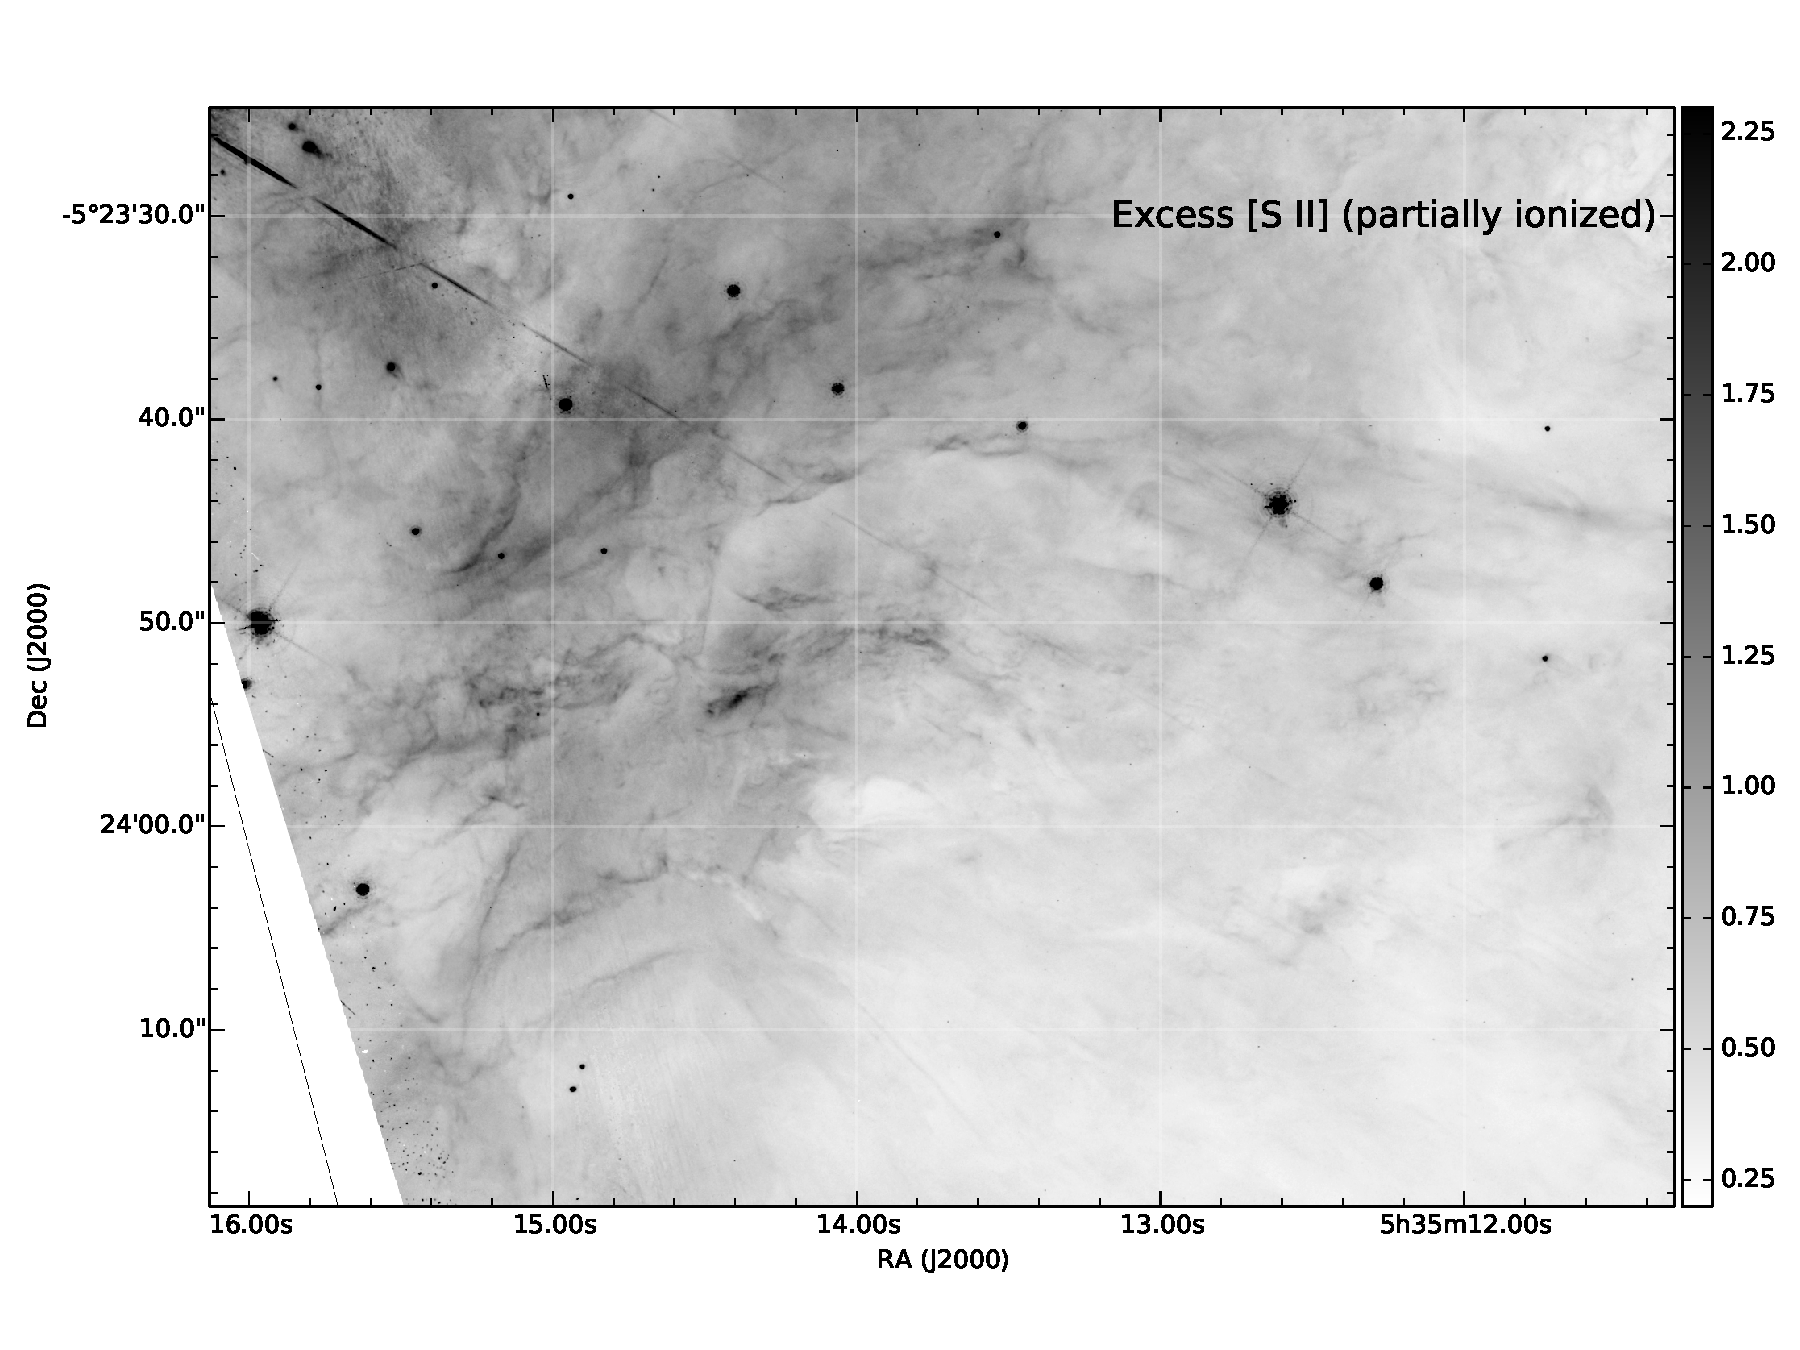
\includegraphics[width=\linewidth]{jet_region_excess-sii}
  \caption{Negative grayscale image of ``excess'' \sii{} emission for
    the same Orion~S region as shown in Fig.~\ref{fig:rgb-jet}.  The
    image was calculated by subtracting a scaled version of the F658N
    image from the F673N image.  This largely cancels out the portion
    of the \sii{} emission that comes from fully ionized gas, leaving
    only the emission from partially ionized gas.  The resulting thin
    filaments trace the positions of ionization fronts and
    low-velocity shocks.  Darker shades correspond to higher surface
    brightness.}
  \label{fig:sii-excess-jet}
\end{figure}

\begin{figure}
  \centering
  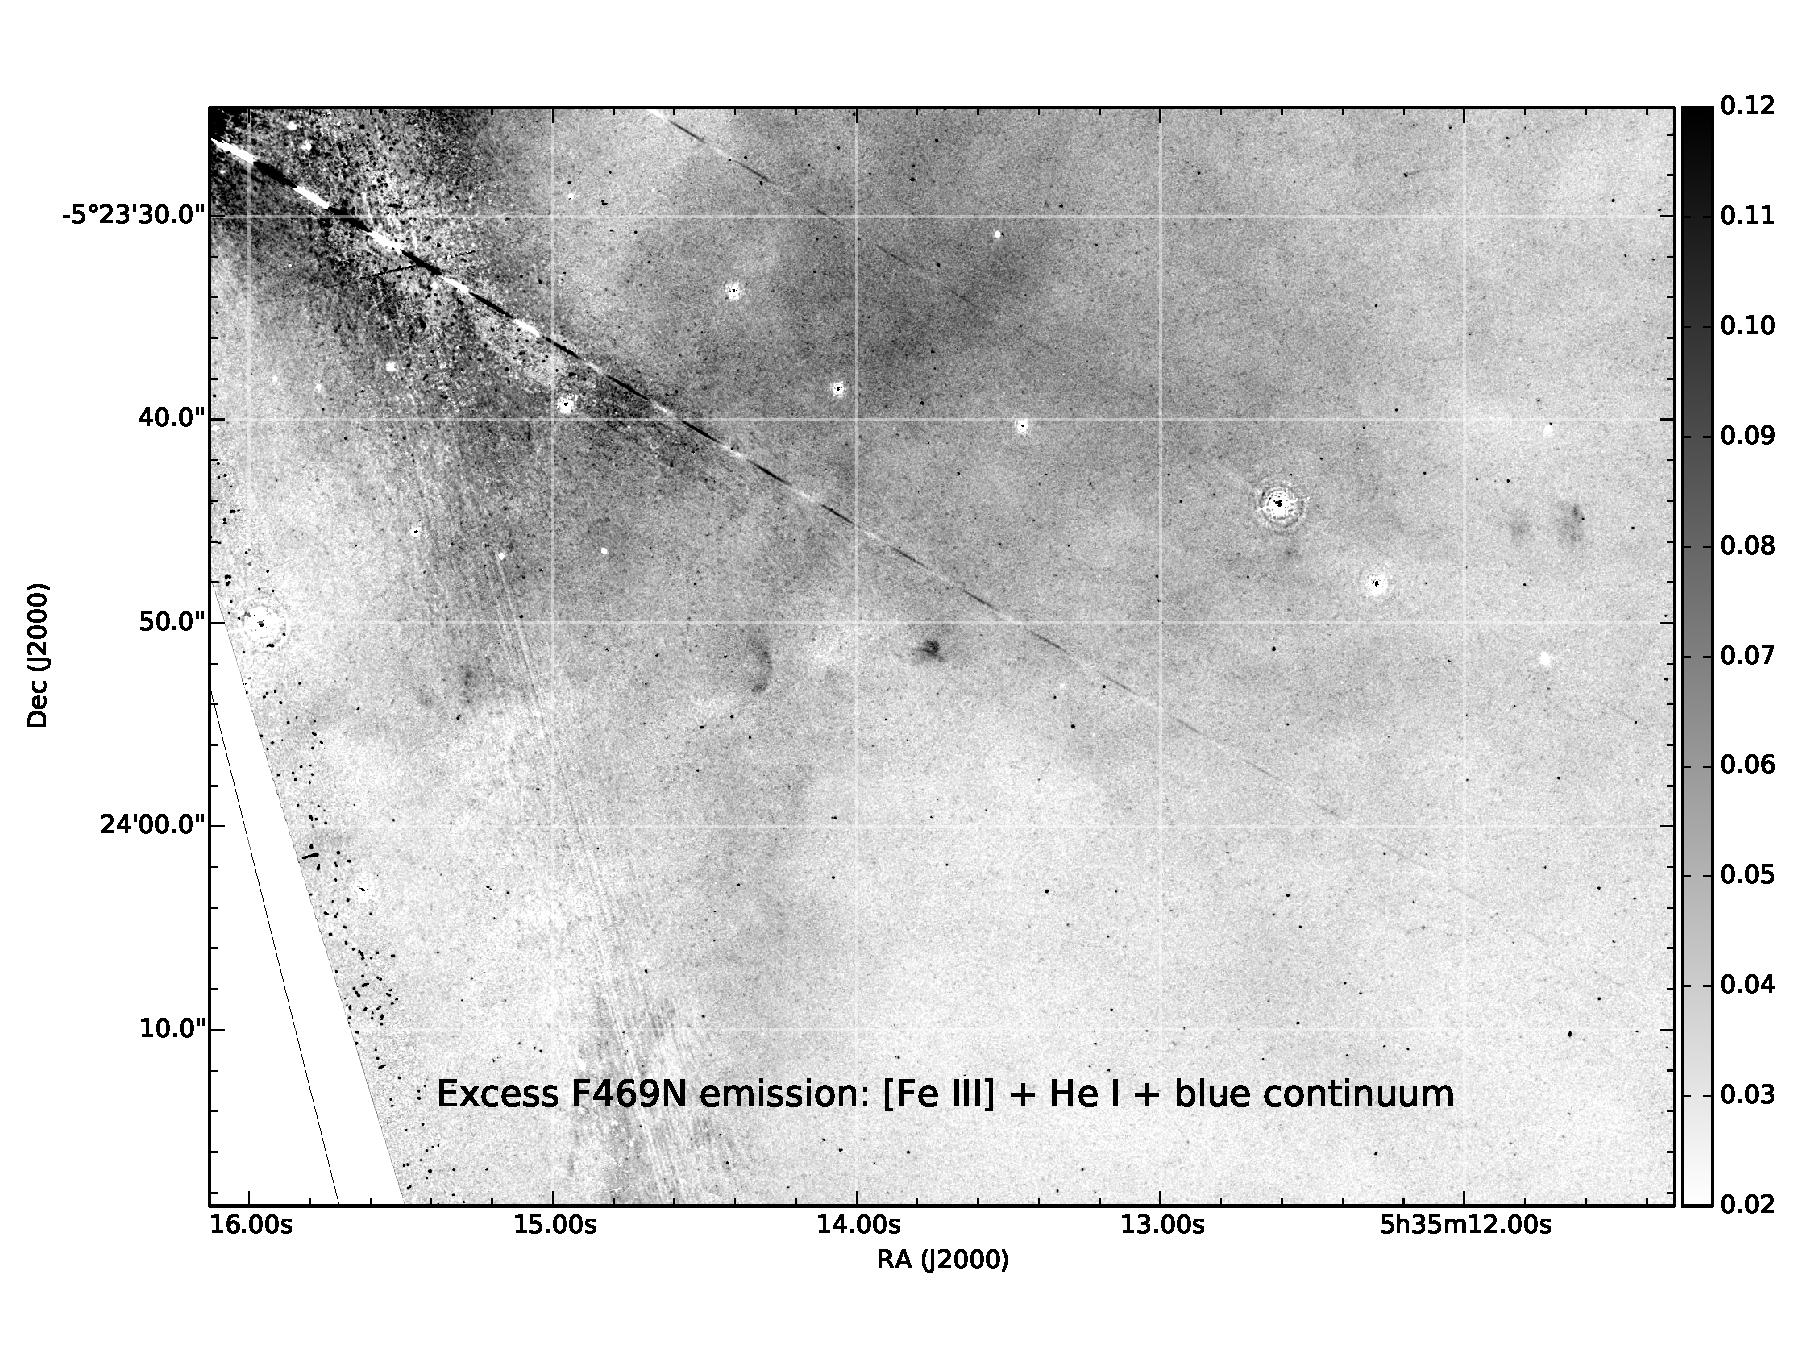
\includegraphics[width=\linewidth]{jet_region_excess-feiii}
  \caption{Negative grayscale image of ``excess'' emission in the
    F469N filter for the same Orion~S region as shown in
    Fig.~\ref{fig:rgb-jet}.  The image was calculated by subtracting a
    scaled version of the F547M continuum image from the F469N image.
    The scaling factor was chosen so as to exactly cancel out the
    continuum contribution to F469N filter for the average spectrum of
    the nebula.  The residual emission is either bluer-than-average
    continuum or due to weak emission lines that fall in the filter
    bandpass (the filter's ostensible target line, \ion{He}{2} 4686,
    is not observed in the Orion Nebula).  The line contribution is
    likely to be due to [\ion{Fe}{3}] 4667+4702, which are extremely
    weak in usual circumstances, but may be considerably enhanced when
    silicate dust grains are destroyed in \(\sim 100~\mathrm{km\
      s^{-1}}\) shocks.}
  \label{fig:feiii-excess-jet}
\end{figure}


\subsection{\boldmath Analysis of fluctuations in \(\Te, \Ne\)}
\label{sec:fluct}

See Figures~\ref{fig:tnii-vs-rad} and~\ref{fig:tsq-nii-vs-binning},
which I need to redo.  Also need to consider density fluctuations.
Provisional conclusion is that the main contribution to true
temperature fluctuations is on rather large scales: 100 linear pixels
or larger (\(> 4''\), \(> 2000\)~AU).  The fluctuations at these
scales are modest: \(t^2 = 0.005\)--\(0.010\).  For the bright inner
regions, there is power in smaller scales, but their global
contribution is small (\(t^2 < 0.003\)) because only a small fraction
of the nebula has small-scale fluctuations, and they may be mainly due
to density fluctuations instead.  For the faint outer regions, there
are essentially zero fluctuations on scales of \(0.4''\)--\(4.0''\),
while the data for scales \(< 0.4''\) are dominated by noise.

\begin{figure}
  \centering
  \begin{tabular}{ll}
    (\textit{a}) & (\textit{b}) \\
    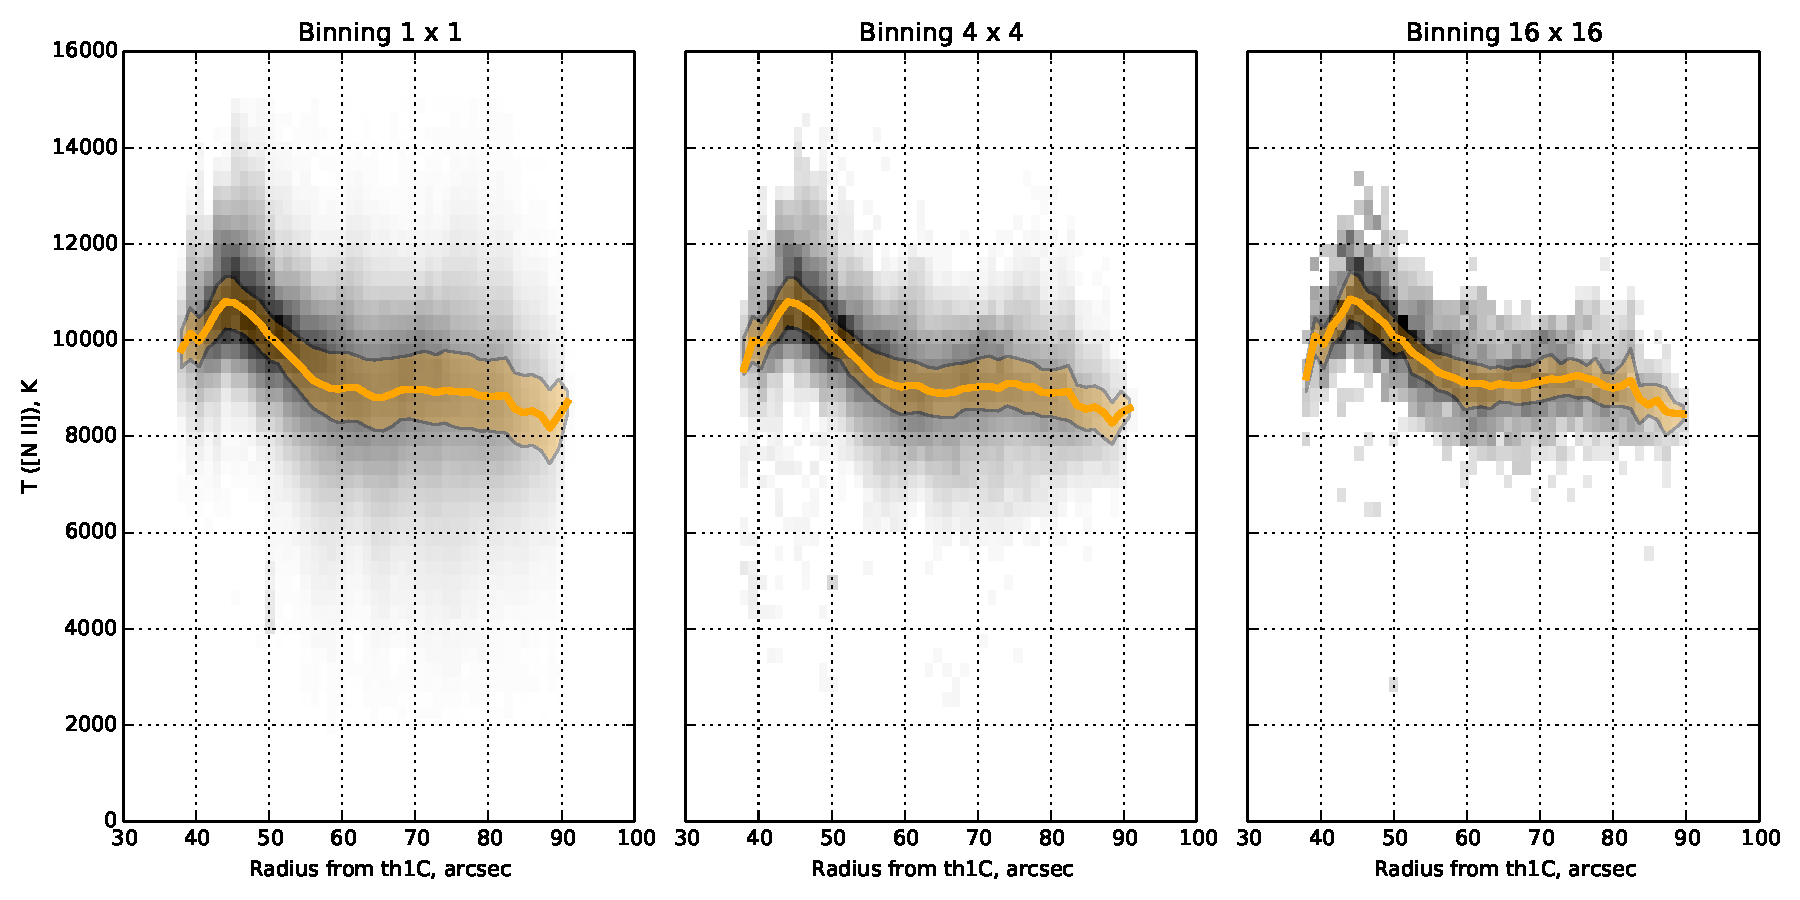
\includegraphics[height=0.35\textheight]{Tnii-vs-radius-binning} &
    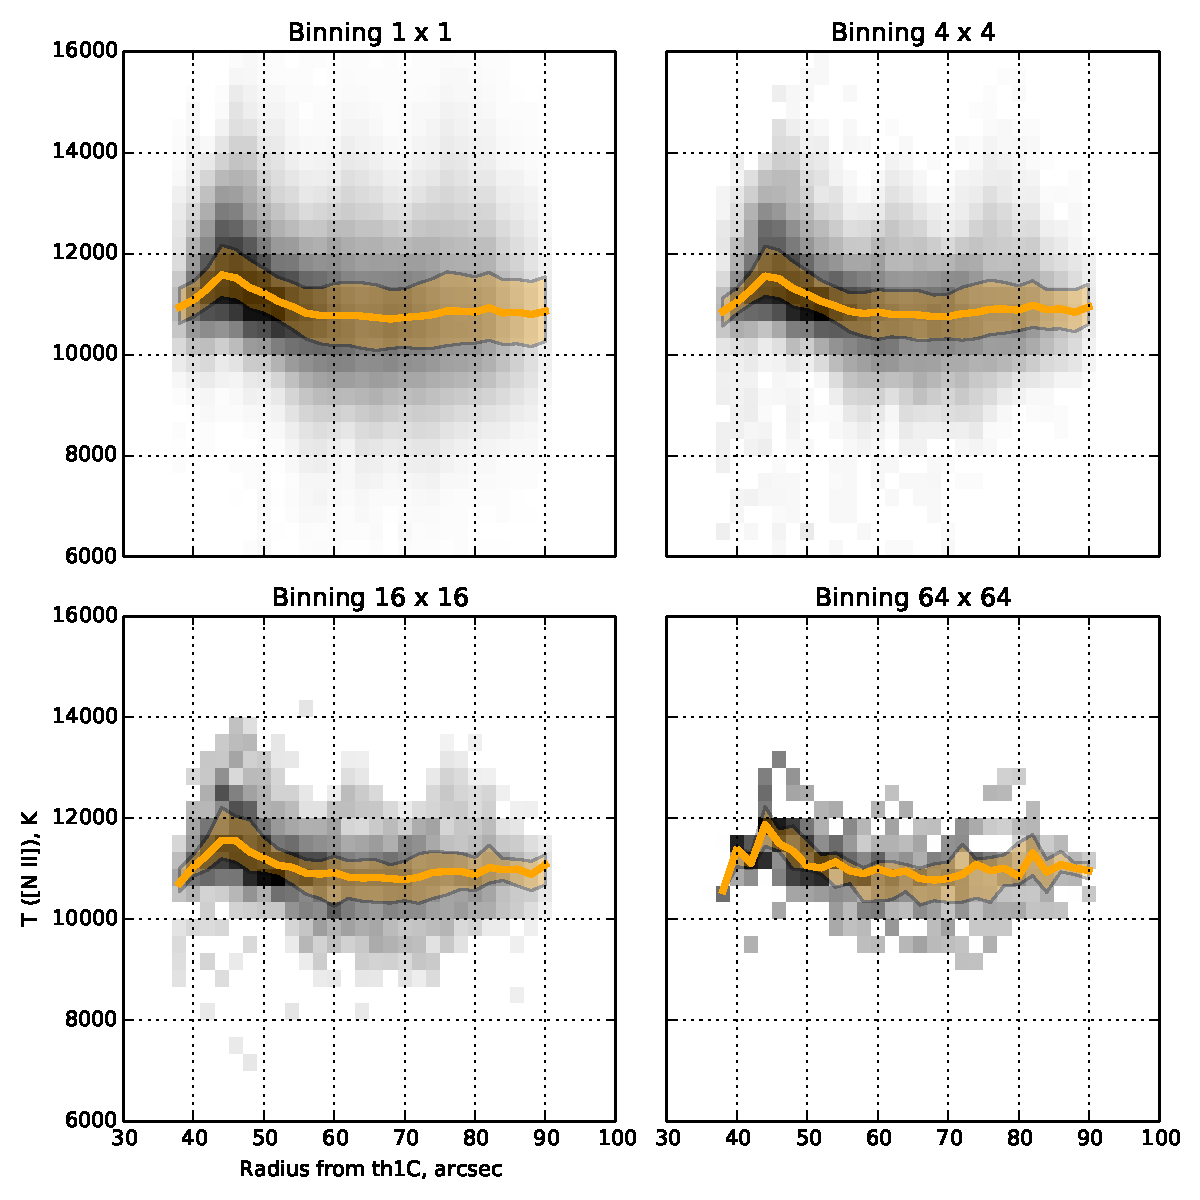
\includegraphics[height=0.25\textheight]{sigma-Tnii-vs-radius-binning}
  \end{tabular}
  \caption{\textit{This still has an old version of the figure.  I
      need to redo it with the new ratios, but the results will likely
      not change.}  (\textit{a})~Temperature distribution as a function of
    radius for different binnings.  (\textit{b})~Standard deviation of
    temperatures as a function of radius for different binnings. 
  }
  \label{fig:tnii-vs-rad}
\end{figure}


\begin{figure}
  \centering

  \begin{tabular}{ll}
    (\textit{a}) & (\textit{b}) \\
    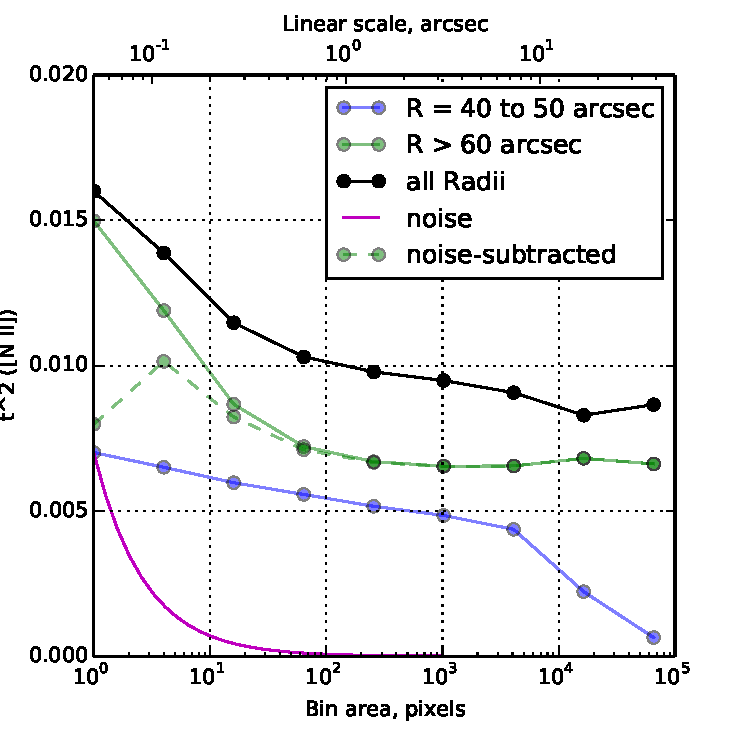
\includegraphics[width=0.45\linewidth]{Tsq-nii-vs-binning-normal} &
    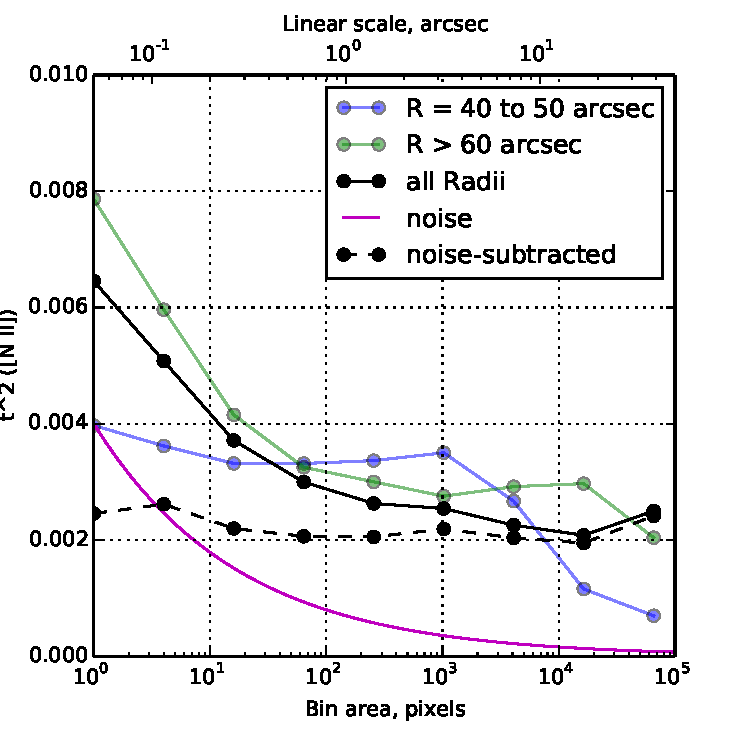
\includegraphics[width=0.45\linewidth]{Tsq-nii-vs-binning-robust}
  \end{tabular}
  \caption{\textit{This still has an old version of the figure.  I
      need to redo it with the new ratios, but the results will likely
      not change.}  Scale-dependence of temperature fluctuations:
    \(t^2\) as a function of binning. (\textit{a})~Variance of
    \(\Te/\bar{\Te}\) for the entire image (black line) and two
    subsamples: an annulus centered on the high-temperature region
    (blue line) and the more distant, fainter regions (green line).
    The magenta line is an estimate of the noise contribution to the
    full sample, and the dashed black line is the result of
    subtracting the noise from the observed values.  (\textit{b})~Same
    as \textit{a} but using a ``robust'' estimator of the variance,
    based on the interquartile range.}
  \label{fig:tsq-nii-vs-binning}
\end{figure}


% \begin{figure}
%   \centering
%   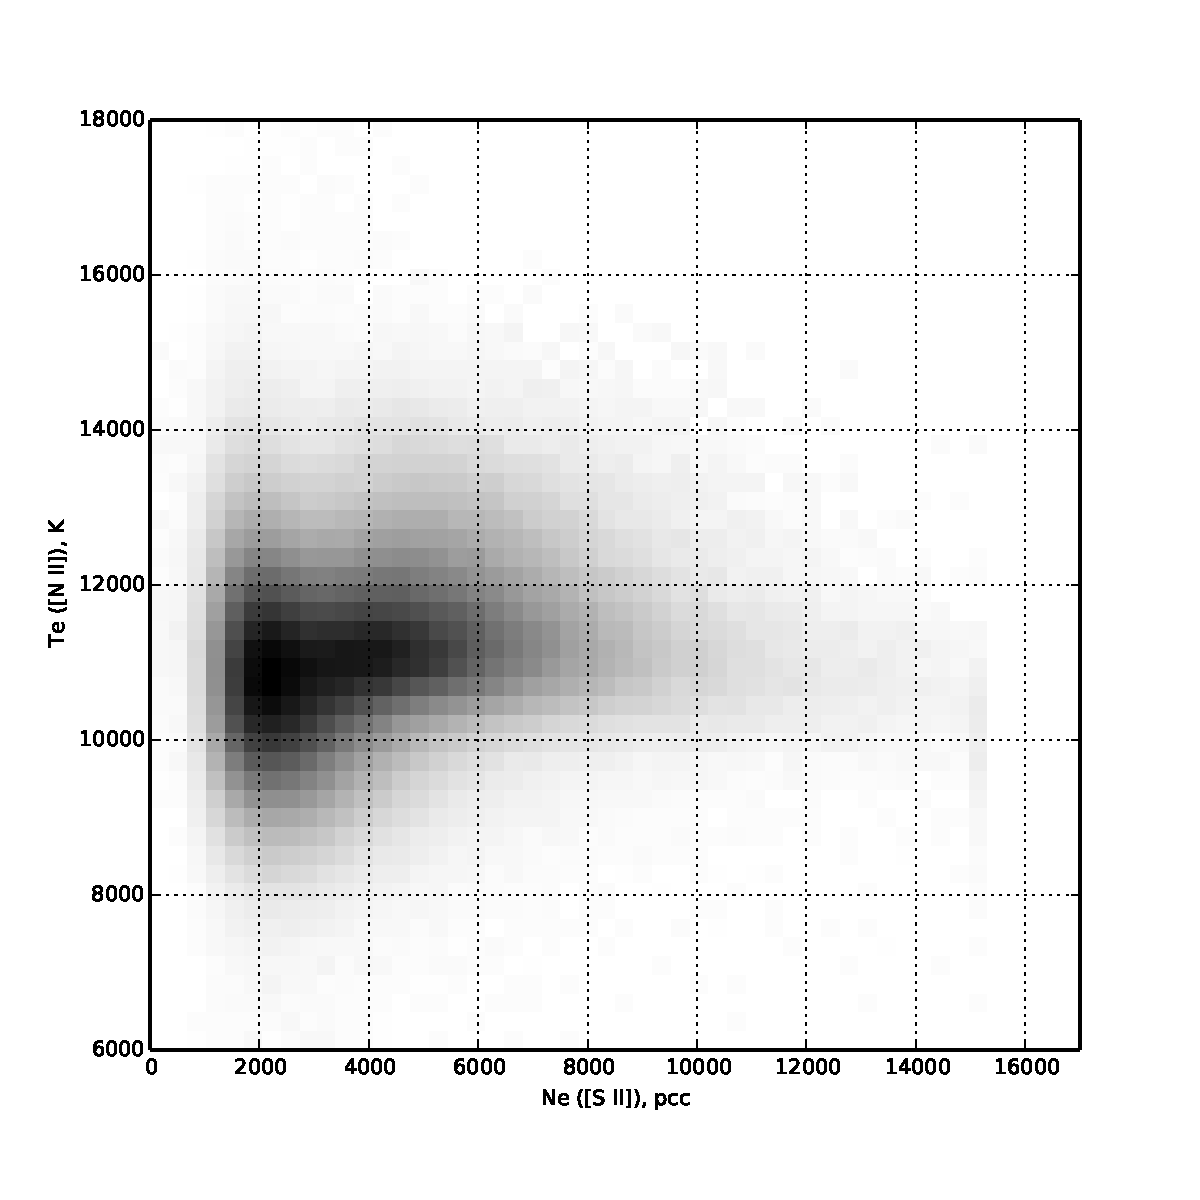
\includegraphics[width=0.8\linewidth]{Te-versus-Ne}
%   \caption{Joint distribution of temperature and electron density for
%     low ionization regions.}
%   \label{fig:Te-Ne}
% \end{figure}

% \begin{figure}
%   \centering
%   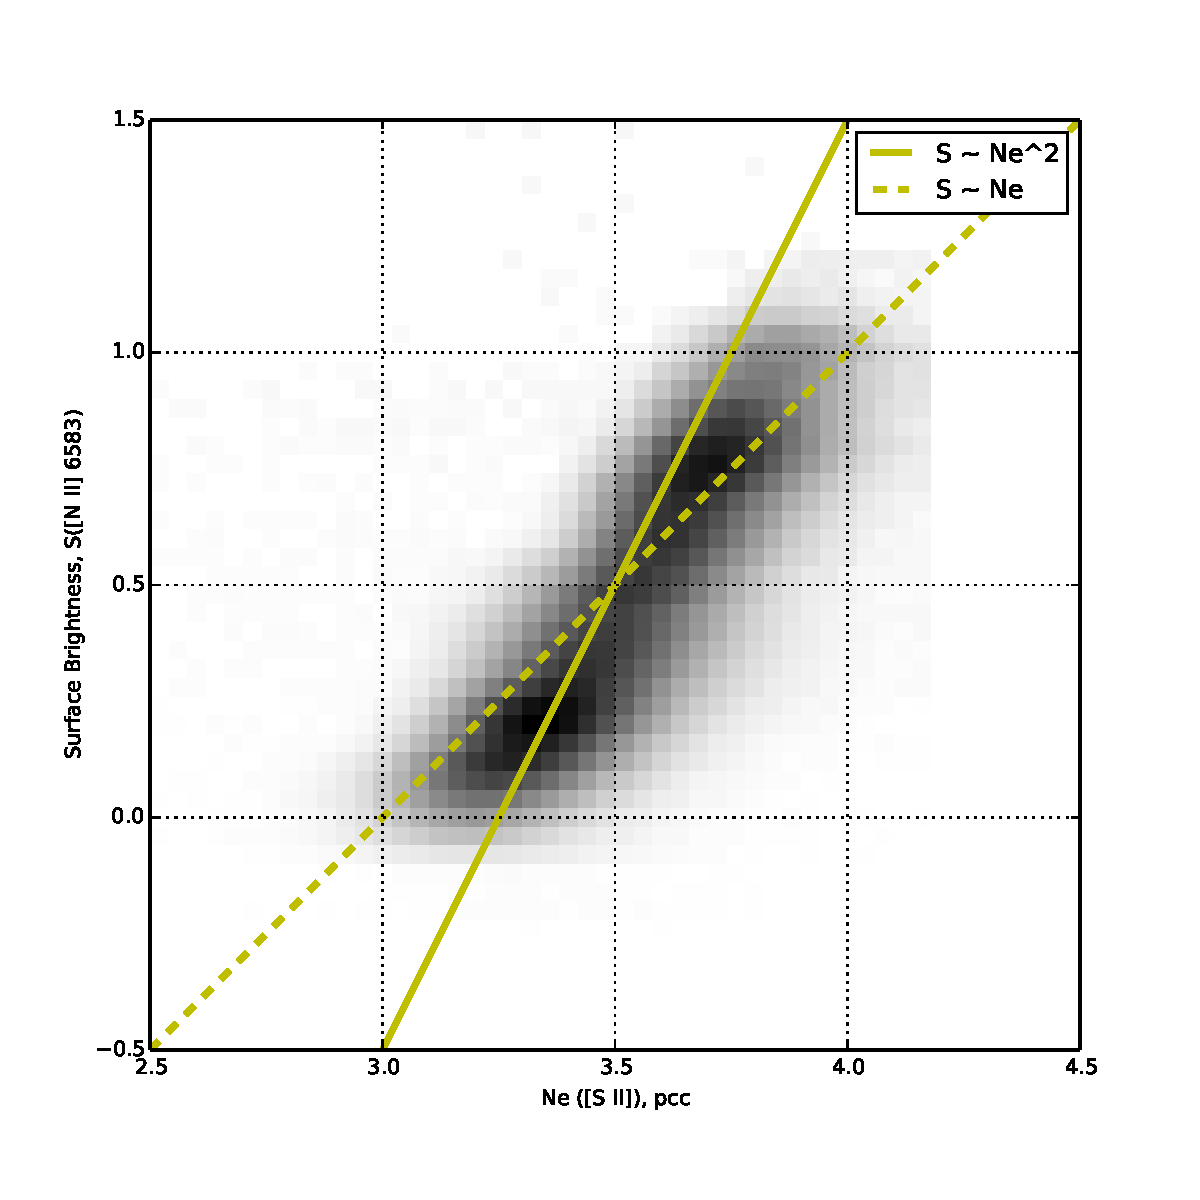
\includegraphics[width=0.8\linewidth]{snii-versus-ne}
%   \caption{Correlation between \sii{} density and \nii{} surface brightness.}
%   \label{fig:Snii-ne}
% \end{figure}


\bibliography{BibdeskLibrary-slavoj}



\appendix

\section{Calibration of the WFC3 filters}

In a recent study \citep{ODell:2013b} of NGC~6720, the Ring Nebula,
evidence was found for significant deviations of some WFC3 UVIS
narrow-band filter calibration constants from the pre-launch
determined values given in the WFC3 Instrument Handbook.  Several
observationally important diagnostic line ratios are significantly
impacted by the filter calibrations in question.  It is therefore of
paramount importance to confirm the calibrations under a wider range
of nebular excitation conditions.  The Orion Nebula, M42, provides an
excellent complement to NGC~6720 in this respect, since it is of lower
ionization and temperature, allowing the calibration to be extended to
smaller values of the emission line equivalent widths, where continuum
contamination of the narrow band filters is greater.  At the same
time, extensive high-quality spectrophotometric data exists for this object,
obtained by distinct teams, using multiple telescopes and instruments
(for example, \citealp{Mesa-Delgado:2008b, ODell:2010a}).  This allows
the true spectrum to be determined with a degree of precision and
confidence that is impossible for other objects.


  % \begin{figure}[p]
  %   \centering
  %   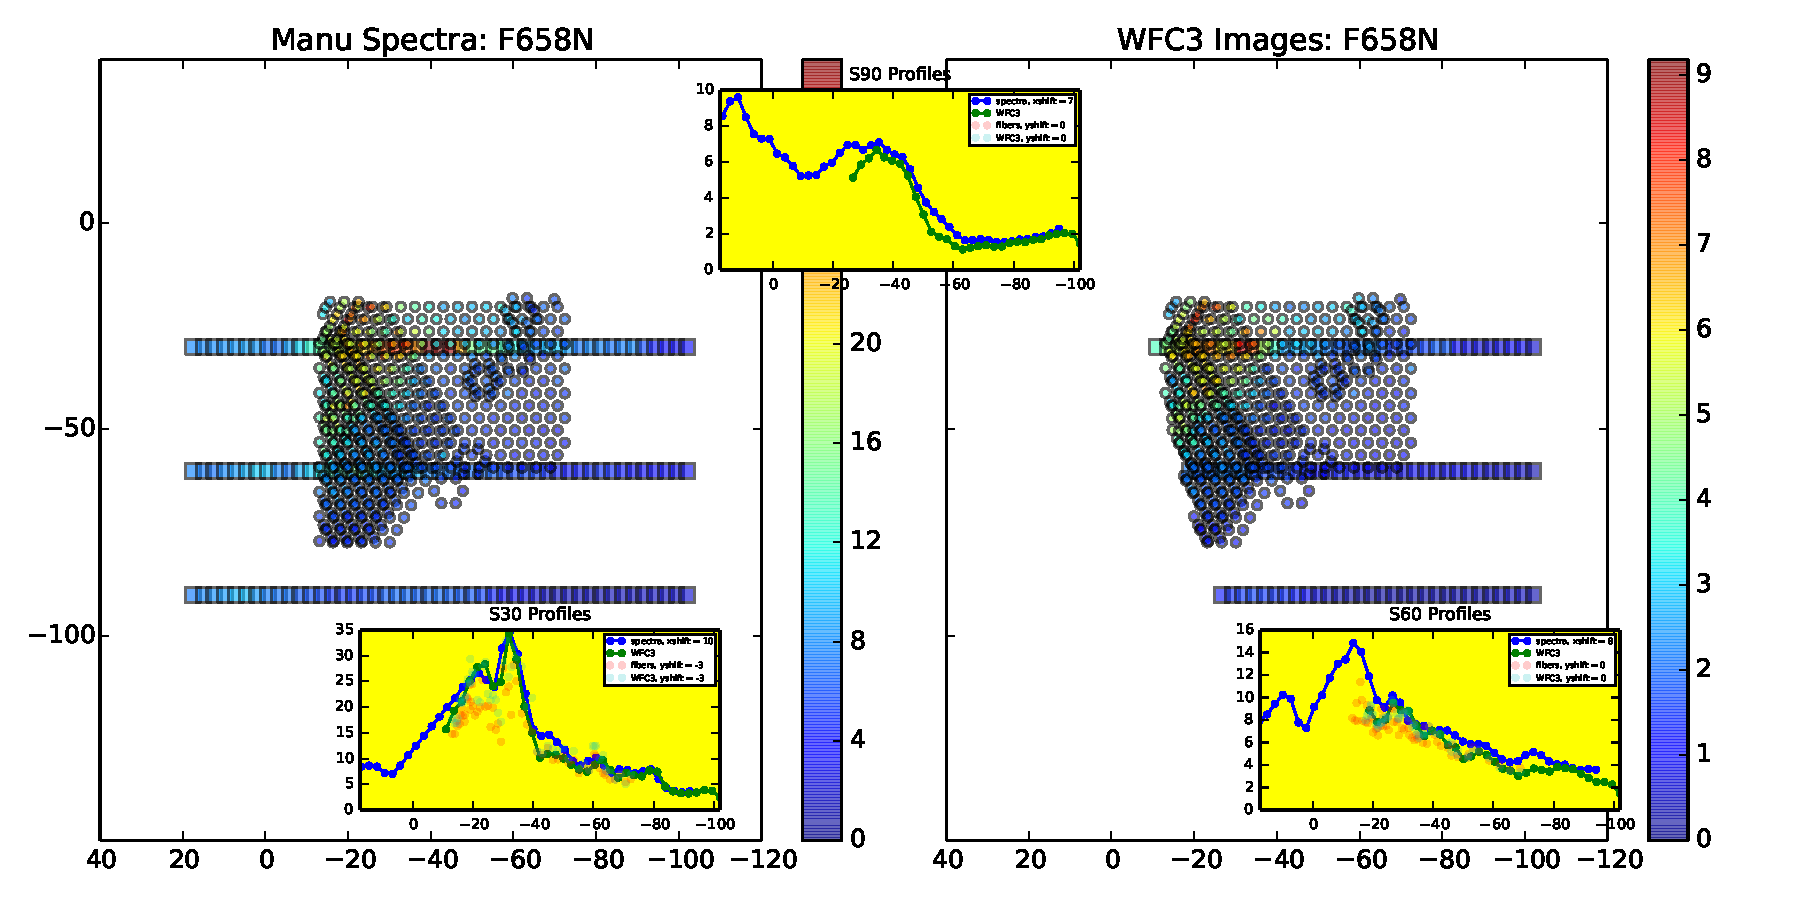
\includegraphics[width=\linewidth]{manu-F658N-red-maps}\\
  %   \includegraphics[width=0.33\linewidth]{odh-F658N-absolute}%
  %   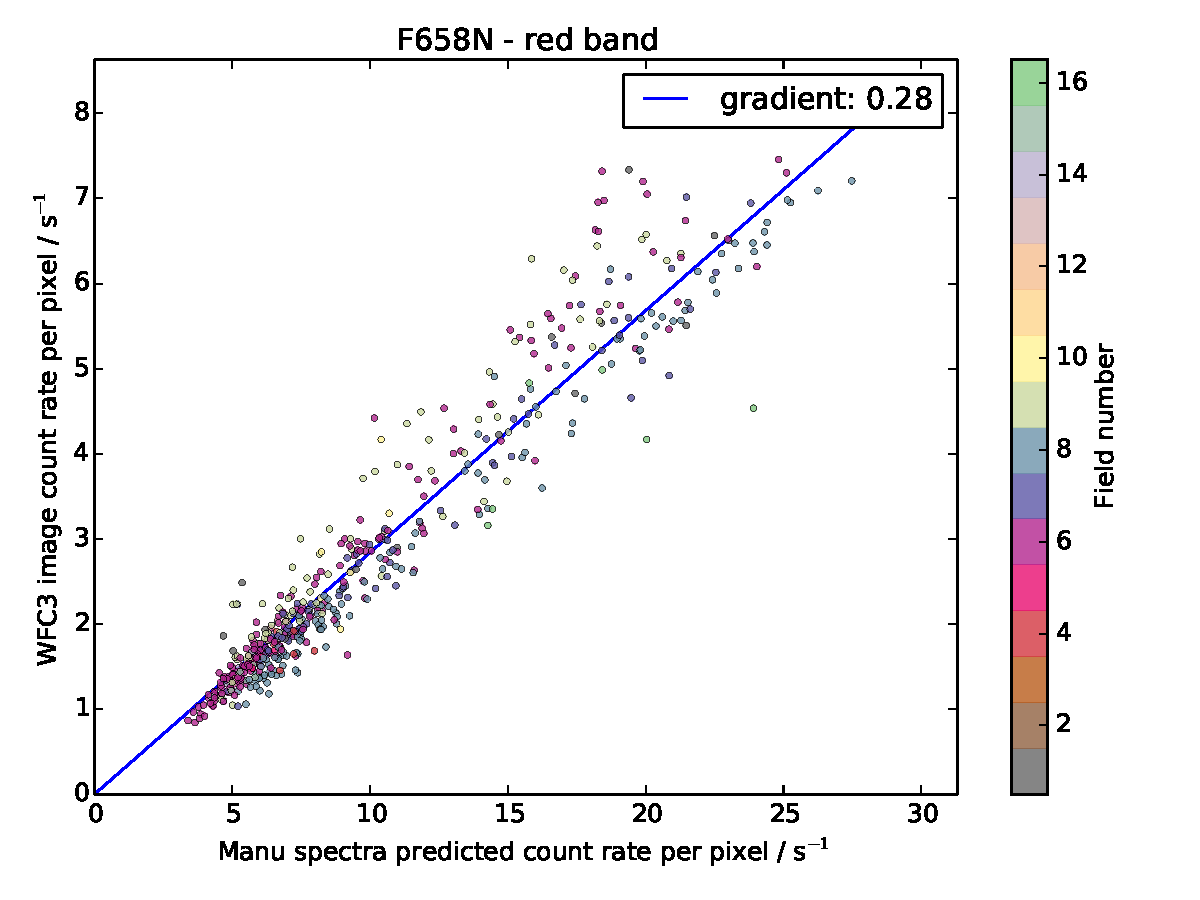
\includegraphics[width=0.33\linewidth]{manu-F658N-red-absolute}%
  %   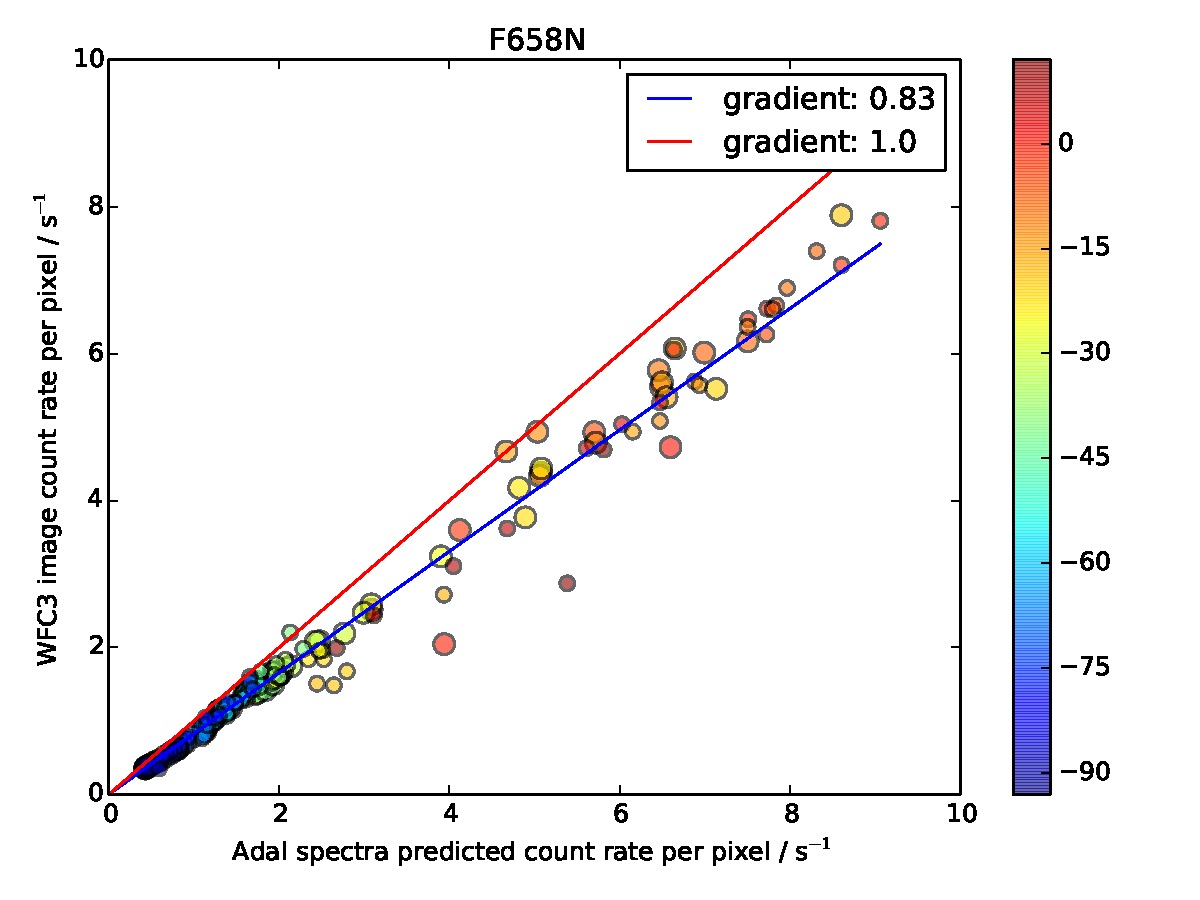
\includegraphics[width=0.33\linewidth]{adal-F658N-absolute}\\
  %   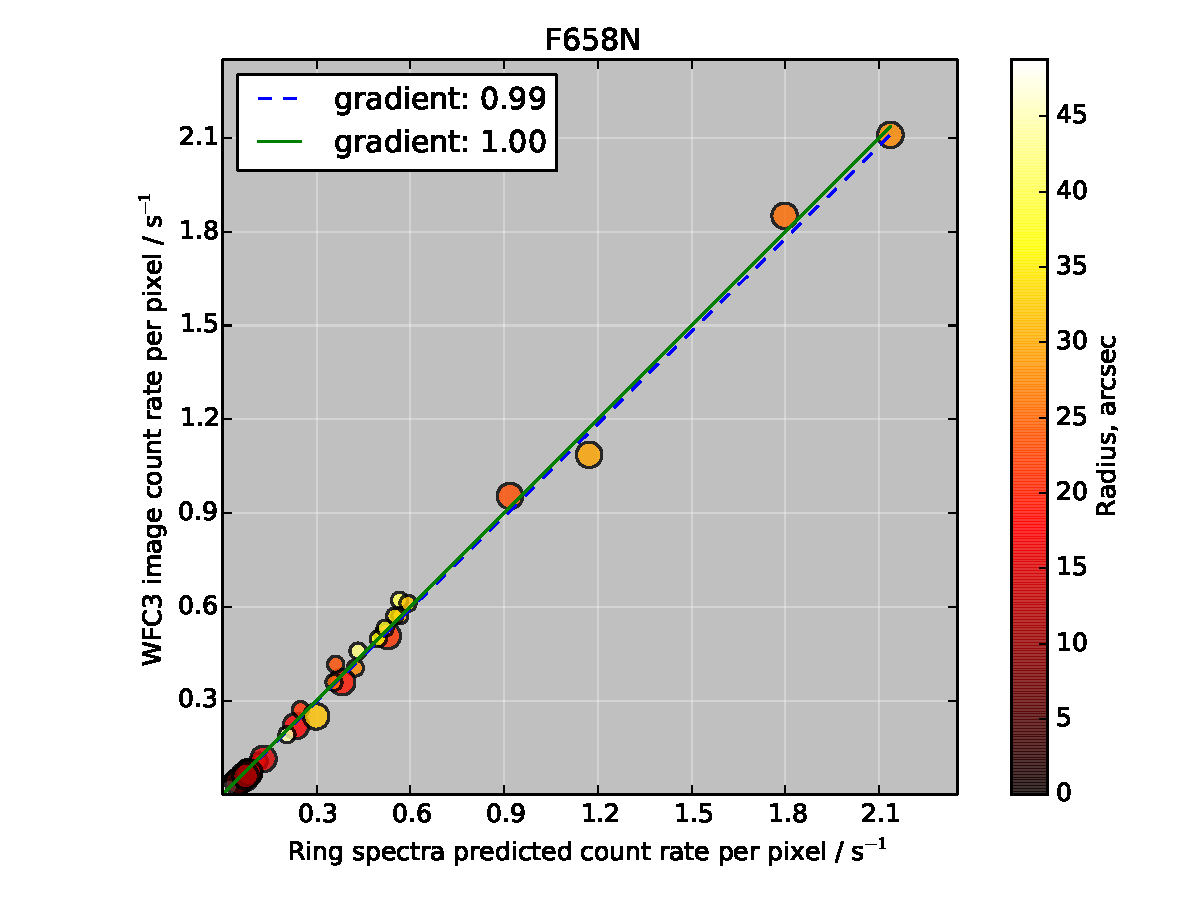
\includegraphics[width=0.33\linewidth]{ring-F658N-absolute}%
  %   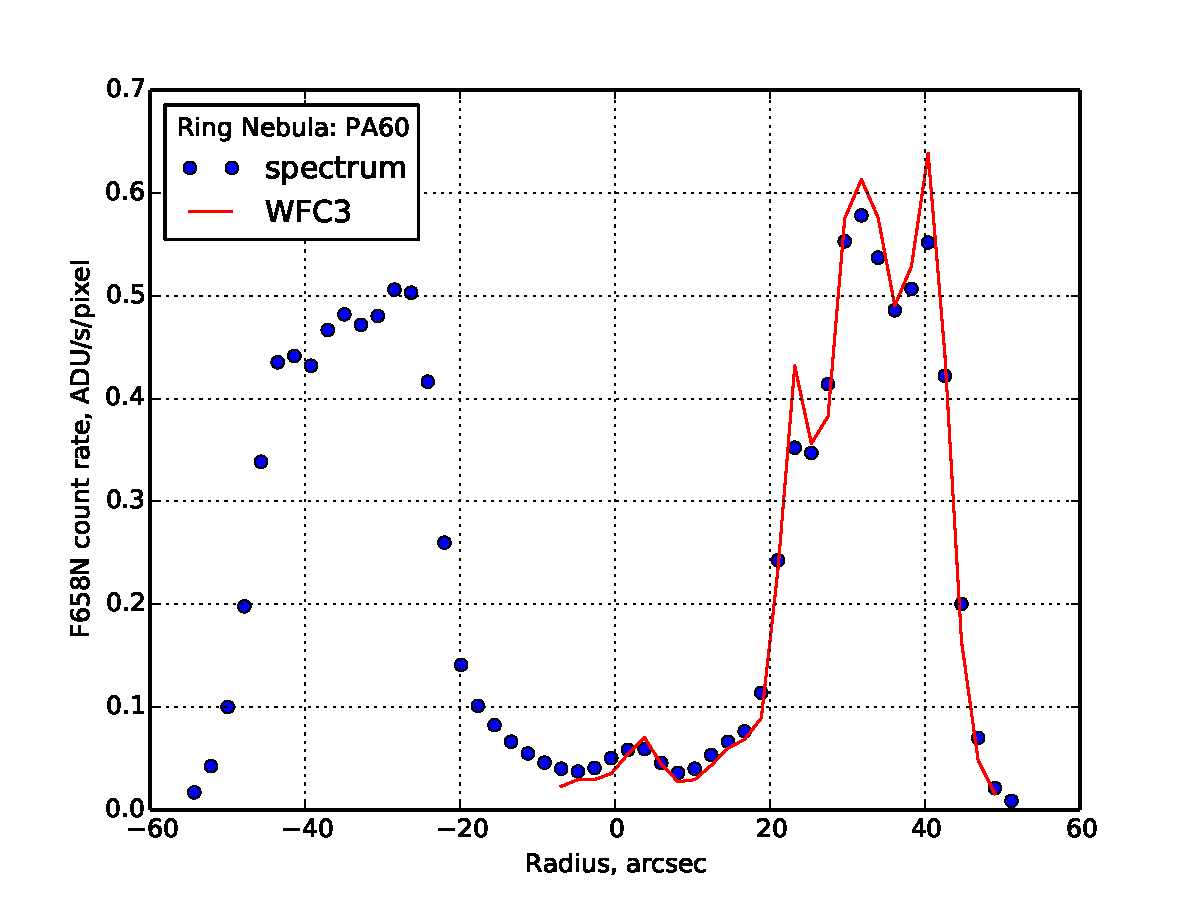
\includegraphics[width=0.33\linewidth]{ring-profile-pa60-F658N}%
  %   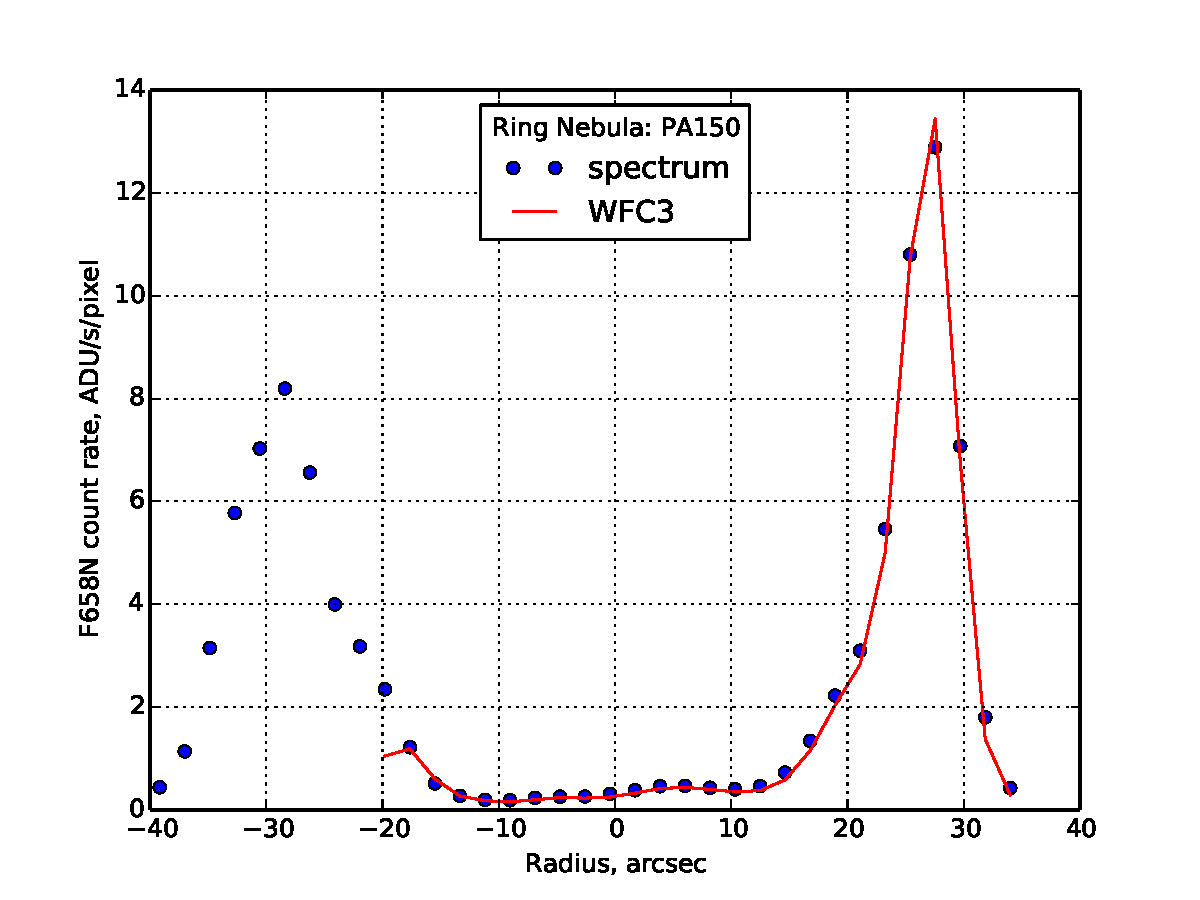
\includegraphics[width=0.33\linewidth]{ring-profile-pa150-F658N}%
  %   \caption{Example of the procedure for spectrophotometrically
  %     calibrating a WFC3 filter.  }
  %   \label{fig:orioncomparison-F658N}
  % \end{figure}

\begin{figure}[t]
  \centering
  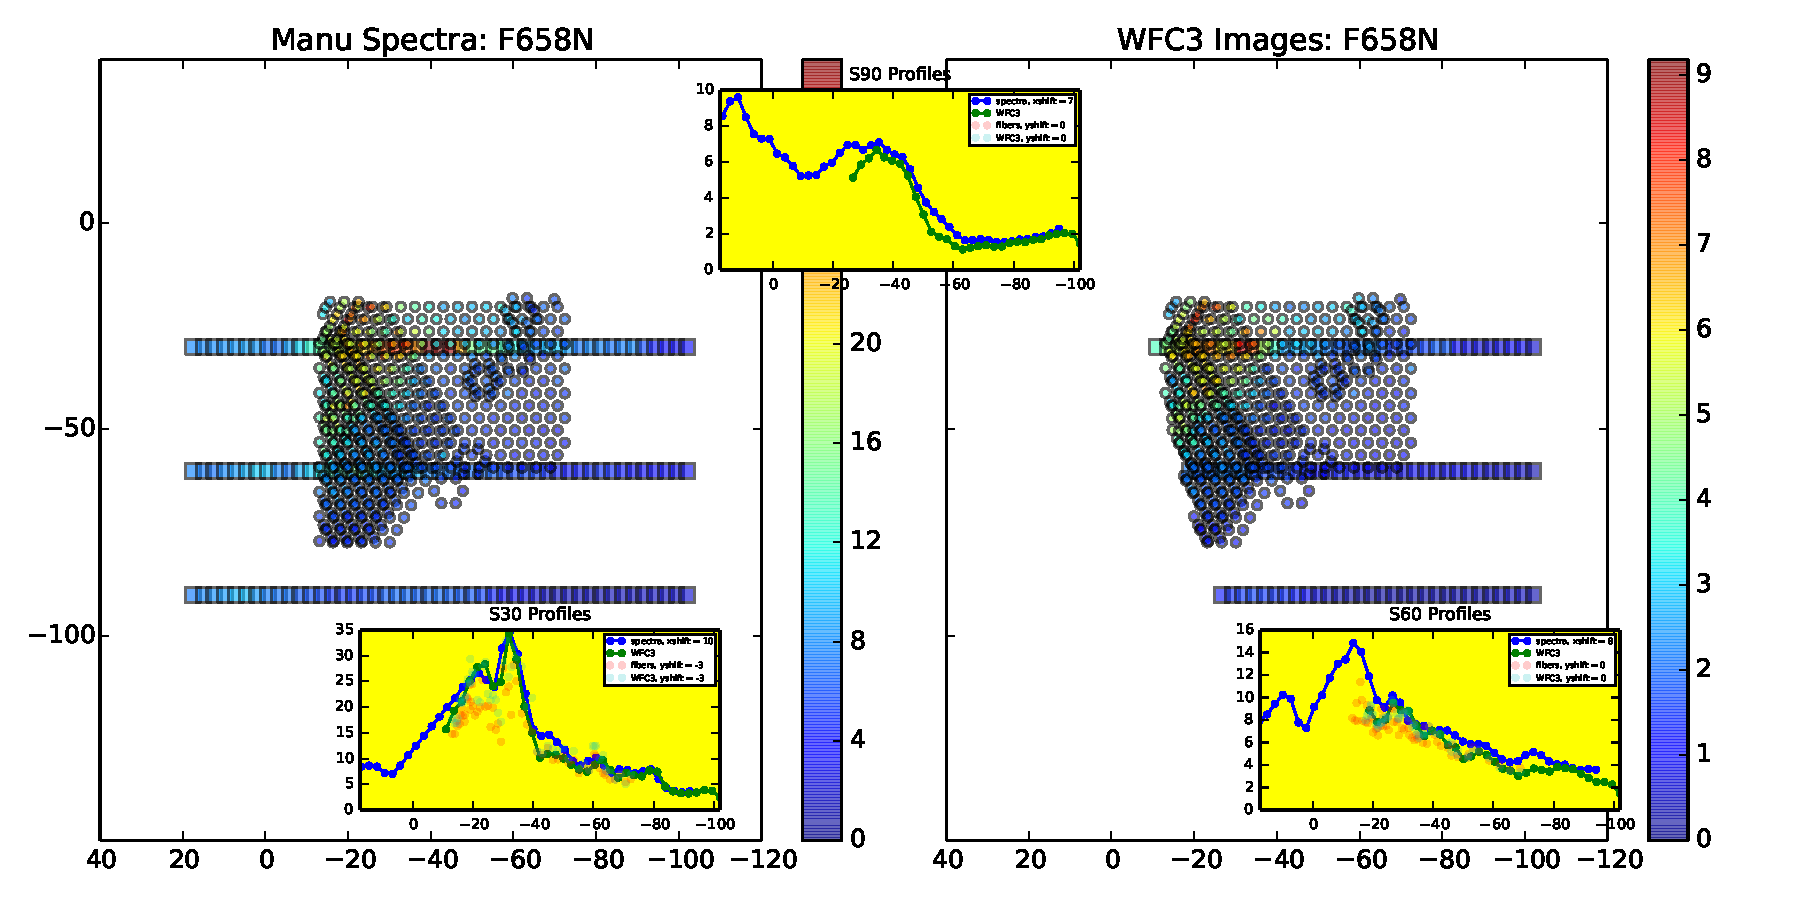
\includegraphics[width=\linewidth]{manu-F658N-red-maps}
  \caption{Example of the procedure for calibrating a WFC3 filter
    using longslit and IFU spectrophotometry of the Orion Nebula.  The
    upper-left panel shows a map of the surface brightness in the
    F658N filter derived from integral field unit observations
    (circles; \citealp{Nunez-Diaz:2013a}) and longslit observations
    (squares; \citealp{ODell:2010a} and triangles;
    \citealp{Mesa-Delgado:2008a}).  In each case, the observed sectrum
    was folded through the nominal filter transmission profile to
    obtain a predicted WFC3 count rate.  The upper-center panel is the
    same, but for the actual WFC3 observations in the F658N filter,
    after smoothing the WFC3 images to the respective ground-based
    resolutions and integrating over a synthetic aperture
    corresponding to each spectrophotometic sample.}
  \label{fig:orioncomparison-F658N}
\end{figure}

\begin{figure}[b]
  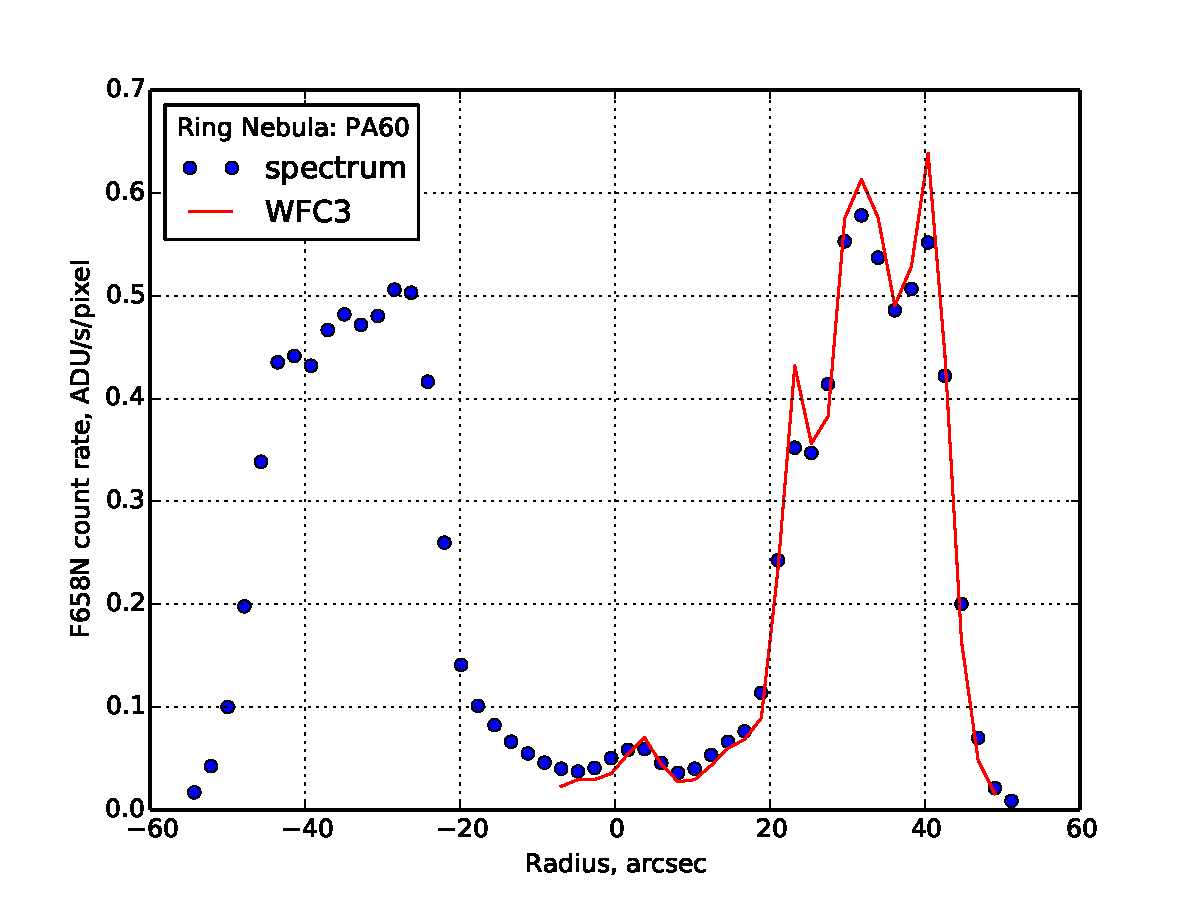
\includegraphics[width=0.5\linewidth]{ring-profile-pa60-F658N}%
  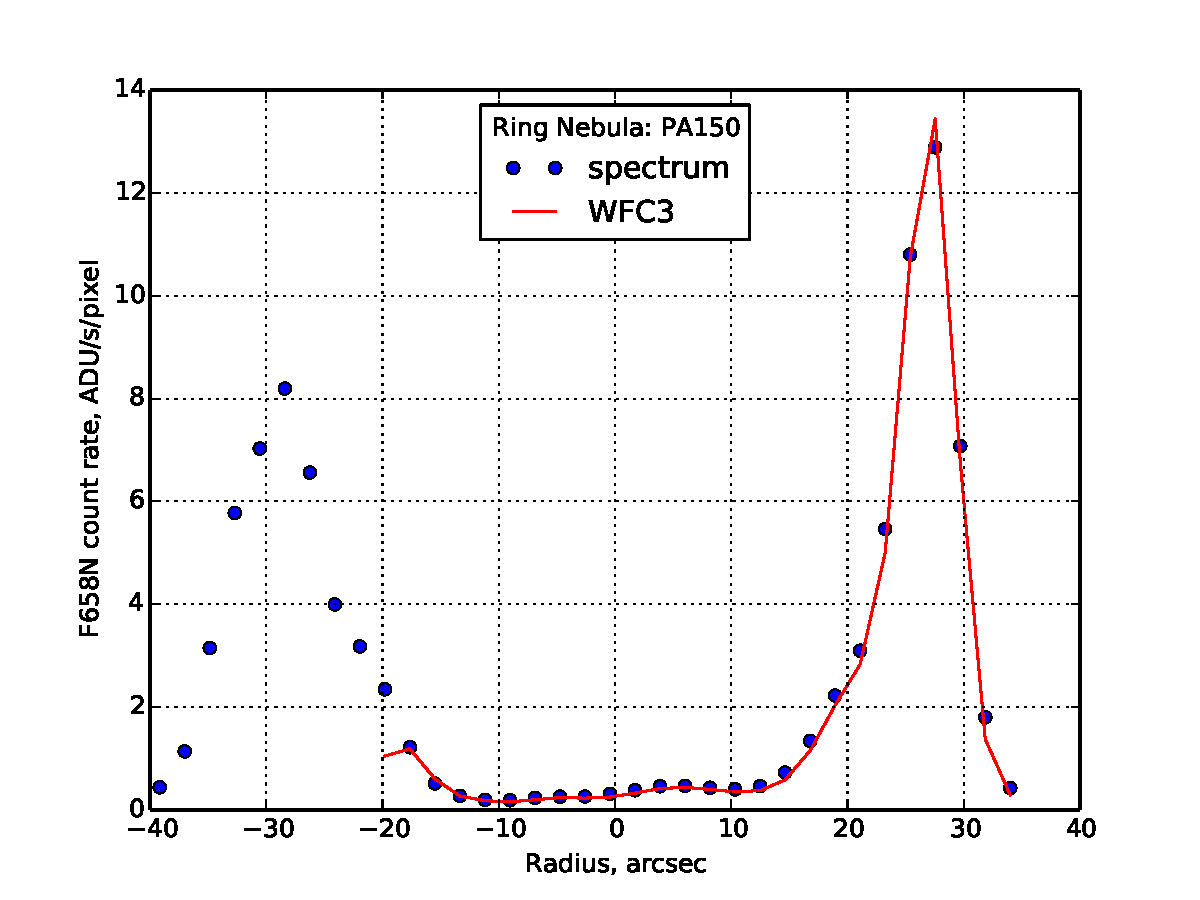
\includegraphics[width=0.5\linewidth]{ring-profile-pa150-F658N}%
  \caption{Example of the procedure for spectrophotometrically
    calibrating a WFC3 filter.  }
  \label{fig:ringcomparison-F658N}
\end{figure}



\newcommand\multicomparison[1]{%
  \raisebox{0.11\linewidth}{#1} & 
  \includegraphics{odh-#1-absolute} &
  \includegraphics{adal-#1-absolute} &
  \includegraphics{ring-#1-absolute} \\
}

\newcommand\tabheader{%
  & Orion: \citet{ODell:2010a}
  & Orion: \citet{Mesa-Delgado:2008b} 
  & Ring Nebula: \citet{ODell:2013b} \\
}

\begin{figure}
  \centering
  \setkeys{Gin}{width=0.3\linewidth}
  \small
  \begin{tabular}{llll}
    \tabheader
    \multicomparison{FQ674N}
    \multicomparison{F673N}
    \multicomparison{FQ672N}
  \end{tabular}
  \caption{Results of spectrophotometric calibration of the nebular
    \sii{} filters of WFC3.  On the vertical axis is plotted the
    observed filter count rate in a series of synthetic apertures that
    coincide with spectrophotometric observations.  On the horizontal
    axis is plotted the predicted count rate calculated by folding the
    observed spectrum through the nominal filter transmission profile.
    The solid line shows a slope of unity, which is what would be
    expected if the nominal throughput were correct.  The dashed line
    shows the best-fit slope. }
  \label{fig:multi-calib-1}
\end{figure}

\begin{figure}
  \centering
  \setkeys{Gin}{width=0.3\linewidth}
  \small
  \begin{tabular}{llll}
    \tabheader
    \multicomparison{F658N}
    \multicomparison{F656N}
    \multicomparison{FQ575N}
  \end{tabular}
  \caption{Same as Fig.~\ref{fig:multi-calib-1} but for the nebular \nii{},  \ha{}, and auroral  \nii{} filters.}
  \label{fig:multi-calib-2}
\end{figure}

\begin{figure}
  \centering
  \setkeys{Gin}{width=0.3\linewidth}
  \small
  \begin{tabular}{llll}
    \tabheader
    \multicomparison{F547M}
    \multicomparison{F502N}
    \multicomparison{F487N}
  \end{tabular}
  \caption{Same as Fig.~\ref{fig:multi-calib-1} but for the green medium-band continuum, nebular \oiii{}, and \hb{} filters. }
  \label{fig:multi-calib-3}
\end{figure}


\begin{figure}
  \centering
  \setkeys{Gin}{width=0.3\linewidth}
  \small
  \begin{tabular}{llll}
    \tabheader
    \multicomparison{F469N}
    \multicomparison{FQ437N}
    \multicomparison{FQ436N}
  \end{tabular}
  \caption{Same as Fig.~\ref{fig:multi-calib-1} but for the \heii{} and auroral \oiii{} filters.}
  \label{fig:multi-calib-4}
\end{figure}






\end{document}
